 \chapter{Introduzione}
\section{Machine learning}

\subsection{Task}
Le \textbf{reti neurali} sono una delle modalità con cui si possono risolvere problemi di \textbf{machine leaning}. Il machine learning è una branca dell'informatica che si occupa di come i computer apprendono e migliorano i propri risultati "imparando" dai loro stessi errori. I computer vengono in particolare applicati a \textbf{task}, i quali possono essere di diversi tipi (classificazione, regressione, clustering, ecc..).

Breve descrizione di alcuni tipi di task:

\begin{itemize}
    \item \textbf{classification}, il task di classificazione è un task \textbf{supervisionato}, il che vuol dire che a partire dalla descrizione e soluzione al problema (training set etichettato), vogliamo imparare un algoritmo di machine learning che crei un modello che risolva task di classificazione del tipo desiderato, in maniera autonoma. In particolare \textbf{il modello deve essere in grado di generalizzare} e predirre correttamente la classe di esempi che non ha visto nella fase di training (esempi: spam detection, sentiment analysis ecc..).
    \item \textbf{regression}, il task di regressione è simile a quello di classifazione, ma invece di predirre un set di lable l'output sarà un numero reale (esempi: house price prediction, stock price prediction ecc..). Si può usare un regressore per fare classificazione.
\end{itemize}


\subsection{No free launch theorem}
In sostanza, questo teorema afferma che a meno di non considerare i bias, gli algoritmi di machine learning sono sostanzialmente uguali in termini di prestazioni.

\subsection{Training di una rete neurale}
Le reti neurali sono una famiglia di incredibilmente flessibili modelli i quali riescono ad approssimare sostanzialmente qualsiasi funzione. Il prezzo da pagare è l'elevatissimo numero di iper parametri grazia ai quali si possono raggiungere ottime performance. Alcuni tipi di iper parametri sono:
\begin{itemize}
    \item numero di layer;
    \item numero di neuroni in ogni layer;
    \item learning rate;
    \item optmizer;.
    \item ....
\end{itemize}


Importantissimo è imparare a settare questi parametri e validare la qualità del modello. Ora ci concentreremo su questi due argomenti.


Il \textbf{generalization error} è l'errore che la nostra funzione \textbf{g} commette quando vede nuovi esempi, è scritta così:
\begin{equation}
    R=E_{(x,y)\sim p^*[L(y,g(x;\Theta))]}
\end{equation}
dove $p^*$ è la \textbf{reale distribuzione dei dati} e 
\begin{equation}
    L(y,g(\cdot;\Theta))
\end{equation}
è la \textbf{loss function} usata per misurare quanto vale l'errore quando $y$ è predetto come $g(x;\Theta)$.

Il problema è che qui $R$ \textbf{non è veramente calcolabile}, non si può fare praticamente. Questo perchè non abbiamo accesso a $p^*$ e anche se ce l'avessimo dovremmo valutare un numero infinito di punti, cosa che non è possibile ovviamente.

Esempi di \textbf{loss function} sono la \textbf{$0-1$ loss}:
\begin{equation}
    L(y,y')=\mathbb{I}_{y\neq y'}=
    \begin{cases}
      1 \text{ if } y\neq y'\\
      0 \text{ otherwise}
    \end{cases}\,
\end{equation}
e la \textbf{quadratic loss}:
\begin{equation}
    L(y,y')=(y-y')^2.
\end{equation}


Tornando a noi, vogliamo misurare il \textbf{generalization error} ma come abbiamo detto ciò richiede un sampling dalla distrubuzione che noi non abbiamo. Per ovviare a questo problema adotteremo diverse soluzioni, la prima è l'utilizzo di un errore diverso dal generalization, un errore più generale detto \textbf{empirical error}:
\begin{equation}
    \hat{R}_T=\dfrac{1}{|T|}\sum_{(x,y)\in T}L(y,g(x;\Theta)),
\end{equation}
dove $T$ è un campione finito estratto da $p^*$.


Arrivati a questo punto:
\begin{itemize}
    \item se  $T$ denota il \textbf{training set}, allora  $T \equiv Tr, \hat{R}_Tr$ denota il \textbf{training error} di $g$,
    \item se  $T$ denota il \textbf{test set}, allora  $T \equiv Te , \hat{R}_Te$ denota il \textbf{test error} di $g$.
\end{itemize}

Siccome il \textbf{training error} è ottimizzato semplicemente con l'algoritmo di apprendimento, ha un \textbf{bias ottimistico} (tende ad essere minore del generalization error). Quindi è sostanzialmente un estimatore ottimistico del generalization error.


Il \textbf{test error} è invece un estimatore \textbf{unbiased} del generalization error $R$, anche se a determinate condizioni il bias può essere \textbf{pessimistico}, per esempio nel caso in cui si tenga da parte una parte del training set (si immagina che trainare il modello una seconda volta utilizzando tutto il training set produca un modello con un errore minore). 


Quando si verifica che l'errore sul test set è maggiore di quello sul training set, cioè
\begin{equation}
    \hat{R}_{Te}-\hat{R}_{Tr} > 0
\end{equation}
si parla di \textbf{overfitting}. A parole, un modello soffre di overfitting quando le prestazioni sul training set sono molto migliori di quelle sul test set. Un leggero overfitting è invece abbastanza normale e tollerabile ma si tende a renderlo più piccolo possibile.\newpage

Tornando invece all'altro dei quesiti inziali, cioè \textbf{come stimare gli iperparametri}; con quello che abbiamo imparato fino ad ora, vogliamo implementare questa procedura: \newline
    redqui ci va il codice python\newline


Sfortunatamente non funziona, per sostanzialmente lo stesso motivo per cui il training è un estimatore ottimistico del generalization erorre, stiamo rendendo anche il test error un estimatore ottimistico. Così facendo stiamo portando il modello a fare overfitting sul test set.



\section{(Matrici e vettori) Calcolo}
\subsection{Derivate}
Data la funzione $y=f(x)$, dove $x$ e $y$ sono numeri reali.
La \textbf{derivata} di $f$ nel punto $x$, denotata da $f'(x)$ or $\frac{df}{dx}(x)$ è la \textbf{pendenza della tangente (o coefficiente angolare)} ad $f$ nel punto $x$.
\begin{figure}[h]
    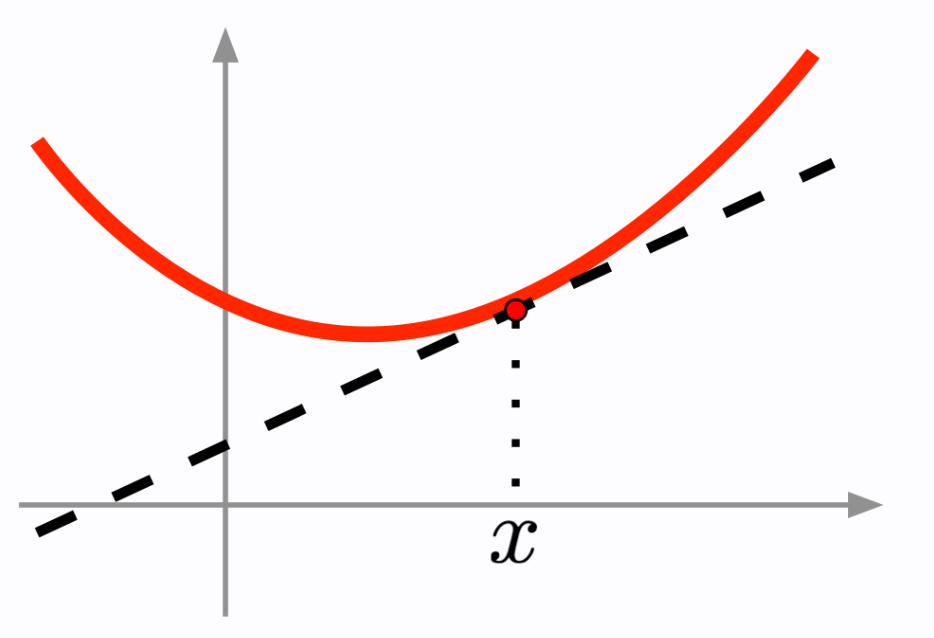
\includegraphics[scale=0.5]{images/prerequisites/derivative.png}
    \centering
\end{figure}
Tra le cose interessanti della derivata c'è il fatto che se si vuole calcolare il valore di $f$ in un punto vicino ad $x$, diciamo $\epsilon$, si può fare in questo modo:
\begin{equation}
    f(x+\epsilon) \approx f(x)+\epsilon f'(x).
\end{equation}

\textbf{Proprietà importanti delle derivate}:
\begin{itemize}
    \item \textbf{linearity} $( \alpha f(x)+ \beta g(x))' = \alpha f'(x)+\beta g'(x)$
    \item \textbf{chain rule} $(f(g(x)))' = f'(g(x))g'(x)$
    \item \textbf{prduct rule} $(g(x)h(x))' = g'(x)h(x)+g(x)h'(x)$
    \item \textbf{quotient rule} $(\frac{f(x)}{g(x)}) = \frac{f(x)'g(x)-f(x)g'(x)}{(g(x))^2}$
    \item \textbf{power rule} $(x^r)' = rx^{r-1}$
\end{itemize}
\newpage
\subsection{Integrali}
Data la funzione $f:\mathbb{R} \rightarrow \mathbb{R}$ e un intervallo $[a,b]$ sulla retta reale: \newline
\textbf{l'integrale di $f$ tra $a$ e $b$ rappresenta l'area sotto $f$ nella regione delimitata dagli estremi dell'intervallo} (quando la funzione si trova sotto lo 0, l'area contribuisce negativamente).
\begin{figure}[h]
    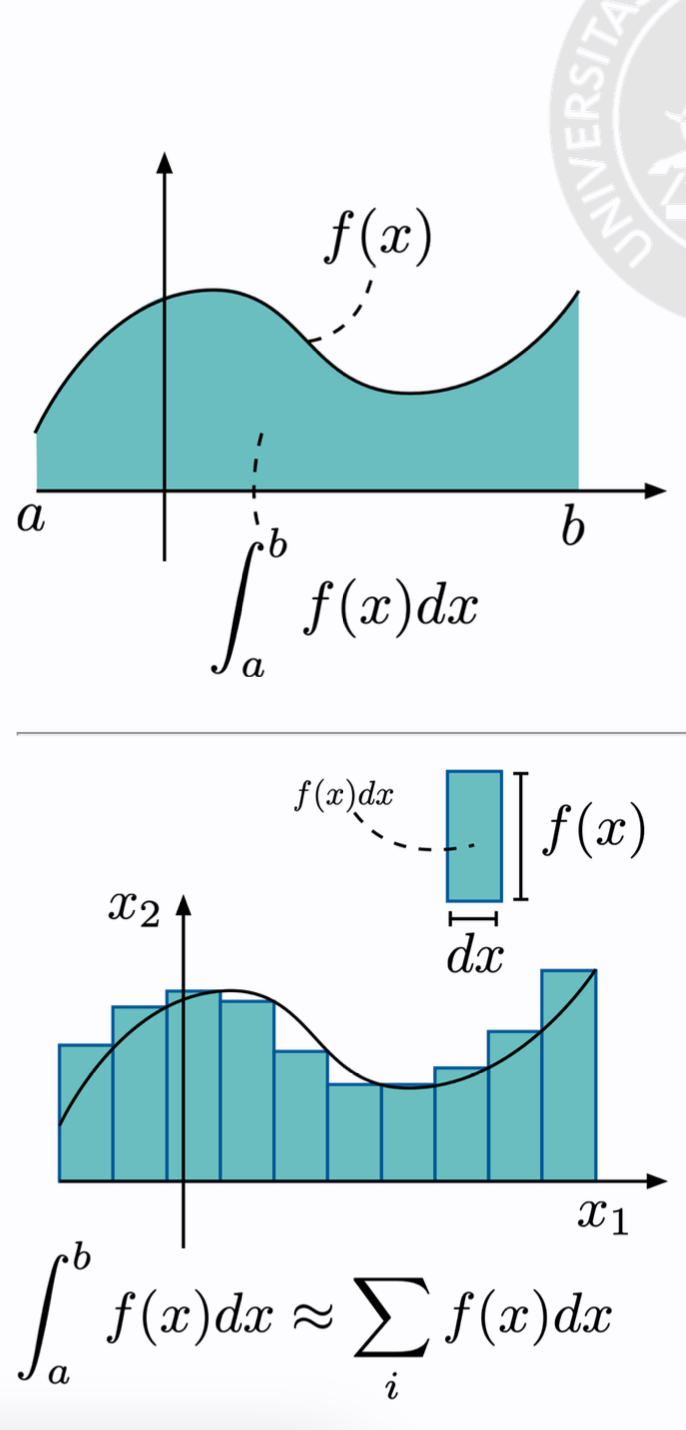
\includegraphics[scale=0.5]{images/prerequisites/integrals.png}
    \centering
\end{figure}
Ciò che è interessante è che esiste un teorema, il \textbf{teorema fondamentale dell'analisi}, che afferma che \textbf{esiste una relazione stretta tra integrali e derivate}. In particolare, se $f$ ammette un'\textbf{antiderivata} $F$, se esiste $F$ tale che $F'(x)=f(x)$ allora:
\begin{equation}
    \int f(x)dx = F(x)+C
\end{equation}
e
\begin{equation}
    \int_a^b f(x)dx = F(x)|_a^b = F(b)-F(a)
\end{equation}

\textbf{N.B.}
\begin{itemize}
    \item gli \textbf{integrali indefiniti} sono quelli per cui \textbf{non è specificato l'intervallo di integrazione} e per cui la soluzione, per convenzione, è l'antiderivata $F$;
    \item gli \textbf{integrali definiti} sono quelli per cui \textbf{è specificato l'intervallo di integrazione}.
\end{itemize}
\newpage
\textbf{Proprietà importanti degli integrali}:
\begin{itemize}
    \item \textbf{linearity} $\int \alpha f(x)+\beta g(x)dx = \alpha \int f(x)dx+\beta \int g(x)dx$
    \item \textbf{constant rule} $\int kdx = kx+C$
    \item \textbf{power rule} $\int x^n dx = \frac{x^{n+1}}{n+1}+C, n \neq-1$
    \item \textbf{log rule} $\int \frac{1}{x}dx = \ln(|x|)+C$
    \item \textbf{exponential rule} $\int a^{kx}dx = \frac{a^{kx}}{k\ln a}+C,x\neq 0$
    \item \textbf{sin rule} $\int \sin(x)dx = -\cos(x)+C$
    \item \textbf{cosin rule} $\int \cos(x)dx = \sin(x)+C$
\end{itemize}

\subsection{Derivate parziali e Gradienti}
Sia data la \textbf{funzione multivariata} $y=f(x_1,\dots,x_n)=f(x)$, dove $y\in \mathbb{R}$,$x\in \mathbb{R}^n$.


La \textbf{derivata parziale} $\frac{\delta}{\delta x_j}f(x)$ \textbf{misura come $f$ varia al variare della sola variabile $x_j$}, tutte le altre rimangono invariate:
\begin{equation}
    \frac{\delta}{\delta x_j}f(x) = \lim_{h \rightarrow 0}\frac{f(x+h\hat{i}_j)-f(x)}{h} = \lim_{h \rightarrow 0}\frac{f(x_1,\dots,x_j+h,\dots,x_n)-f(x_1,\dots,x_n)}{h}
\end{equation}
\begin{figure}[!h]
    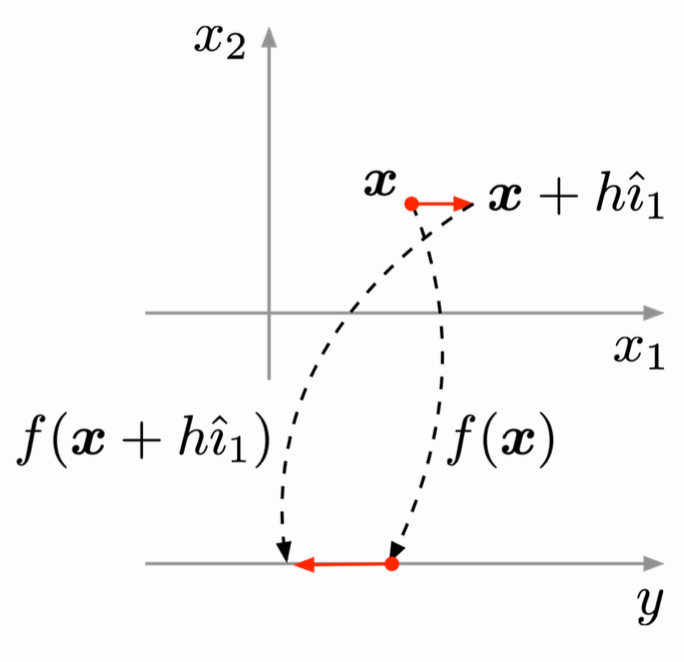
\includegraphics[scale=0.5]{images/prerequisites/partDerivatives.png}
    \centering
\end{figure}
\newline
Il \textbf{gradiente} di $f$, denotato con $\nabla_xf$ (o più semplicemente $\nabla f$) è \textbf{il vettore che contiene tutte le derivate parziali della funzione $f$}:
\begin{equation}
    \nabla f=\left[\frac{\delta f}{\delta x_1},\dots,\frac{\delta f}{\delta x_n}\right]^T.
\end{equation}
Il gradiente è un vettore con una proprietà molto particolare, per parlare della quale bisogna introdurre prima un concetto: \textbf{la regola della catena per il calcolo multivariato}.


Assumiamo $z=f(x,y)$ e siano $x,y$ variabili dipendenti da una variabile addizionale $t$ (gli input di $f$ sono a loro volta funzioni della variabile $t$, cioè abbiamo $f(x(t),y(t))$), quindi:
\begin{equation}
    \frac{dz}{dt}=\frac{\delta z}{\delta x}\frac{dz}{dt}+\frac{\delta z}{\delta y}\frac{dy}{dt}.
\end{equation}
Quello appena visto vale per 2 variabili, più in generale per $f:\mathbb{R}^n\rightarrow \mathbb{R}$, quando $x_1,\dots,x_n$ dipendono da una variabile $t$:
\begin{equation}
    \frac{df}{dt}=\sum^n_{i=1}\frac{\delta f}{\delta x_i}\frac{dx_i}{dt}.
\end{equation}
\newpage
Facciamo un esempio, date:

\begin{itemize}
    \item $(x,y)=(t^2,t)$, perciò $x(t)=t^2$ e $y(t)=t$;
    \item $z=f(x,y)=x^2y^2$
\end{itemize}
calcolare le derivata di $z$ rispetto a $t$. 
Cioè:
\begin{equation}
    \frac{\delta z}{\delta t}=\frac{\delta z}{\delta x}\frac{dx}{dt}+\frac{\delta z}{\delta y}\frac{dy}{dt}=2xy^2\cdot 2t+2x^2\cdot1=4t^5+2t^5=6t^5.
\end{equation}

\subsection{Derivate direzionali}
Vediamo ora un'applicazione immediata della regola della catena nel caso multivariato. Fino ad ora abbiamo calcolato la derivata soltanto lungo gli assi ma cosa succede se invece scegliamo di calcolarla lungo un vettore qualsiasi? Qual è il tasso di variazione della funzione rispetto al movimento in una direzione data da un vettore?


Sia $u$ un vettore unità. La derivata direzionale di $f$ nel punto $x$ nella direzione di $u$ è esattamente il \textbf{tasso di cambiamento nella direzione indicata dal vettore $u$}.
\begin{equation}
    D_uf(x)=\lim_{h\rightarrow 0}\frac{f(x+hu)-f(x)}{h}
\end{equation}
\begin{figure}[!h]
    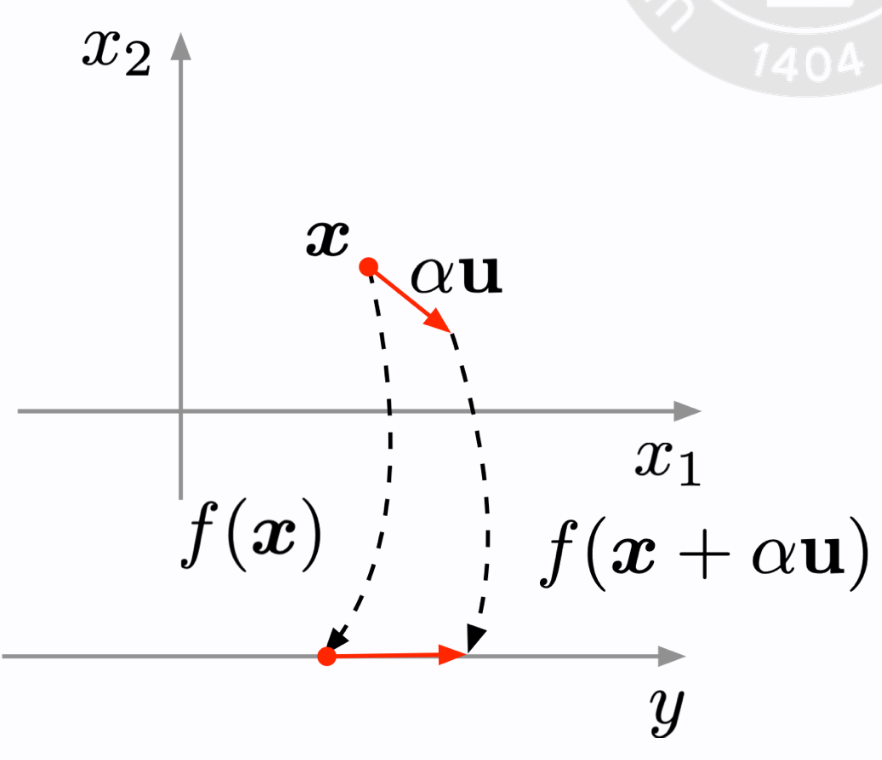
\includegraphics[scale=0.5]{images/prerequisites/dirDerivatives.png}
    \centering
\end{figure}



In altre parole, la derivata direzionale è la derivata di $f(x+\alpha u)$ rispetto ad $\alpha$ calcolata quando $\alpha = 0$.


Utilizzando la \textbf{chain rule}, possiamo facilmente calcolare un'espressione per $D_uf(x)$:
\begin{equation}
    D_uf(x)=\frac{d}{d\alpha}(x+\alpha u)\Big|_{\alpha=0}=\sum^n_{i=1}\frac{\partial f(x+\alpha u)}{\partial x_i}\Big|_{\alpha = 0}\frac{dx_i}{d\alpha}=\nabla f(x)\cdot u = u^T\nabla f(x).
\end{equation}

\newpage
Ci interessa ora \textbf{trovare la direzione nella quale la funzione cresce maggiormente}, ovvero trovare $u$ tale che $D_uf$ è maggiore. Vogliamo risolvere:
\begin{equation}
    \max_{u,u^Tu=1}D_uf(x)=\max_{u,u^Tu=1}u^T\nabla f(x)=\max_{u,u^Tu=1}|u||\nabla f(x)|cos(\theta).
\end{equation}
\begin{figure}[!h]
    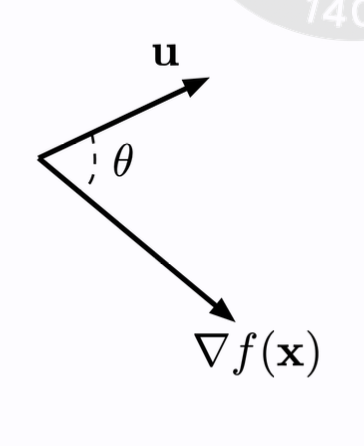
\includegraphics[scale=1]{images/prerequisites/maxGradient.png}
    \centering
\end{figure}



Ora, visto che $|u|=1$ e $\nabla f(x)$ non dipende da $u$, ciò che ci rimane è cercare $u$ tale che massimizzi il $cos(\theta)$. Questo implica però che \textbf{il massimo viene raggiunto quando $u$ ha la stessa direzione di $\nabla f(x)$}.
\newline

\textbf{IMPORTANTE: il gradiente punta nella direzione nella quale $f$ cresce di più}.
\newpage

\subsection{Matrice Jacobiana}
Quando abbiamo una funzione che oltre ad essere multivariata \textbf{ha anche molti output diversi}:
\begin{equation}
    f:\mathbb{R}^n\rightarrow \mathbb{R}^m, f(x)=[f(x)_1,\dots,f(x)_m]^T
\end{equation}
se calcoliamo tutte le derivate di un oggetto di questo tipo, stiamo calcolando lo \textbf{Jacobiano della funzione $f$}. Più formalmente essa è la matrice $J\in \mathbb{R}^n\rightarrow \mathbb{R}^m$ che contiene tutte le derivate parziali di $f(x_i),(1\leq i \leq m)$ per tutte le variabili $x_j,(1\leq j \leq n)$:
\begin{equation}
    J_{i,j}=\frac{\partial}{\partial x_j}f(x)_i
\end{equation}
o, equivalentemente, lo Jacobiano è la matrice contenente $\nabla[f(x)_i]$ nella riga $i-esima$:
\begin{equation}
    J=[\nabla[f(x)_i]^T]^m_{i=1}.
\end{equation}

\subsection{Derivate seconde}
La \textbf{derivata seconda} è la derivata di una derivata. Per esempio, sia $\mathbb{R}^n\rightarrow \mathbb{R}$, possiamo calcolare $n^2$ derivate seconde:
\begin{equation}
    \frac{\partial^2}{\partial x_i\partial x_j}f(x).
\end{equation}
La derivata seconda ci dice \textbf{come cambia la derivata prima al variare dell'input}. Può anche essere vista come una \textbf{misura della curvatura}.
\begin{figure}[!h]
    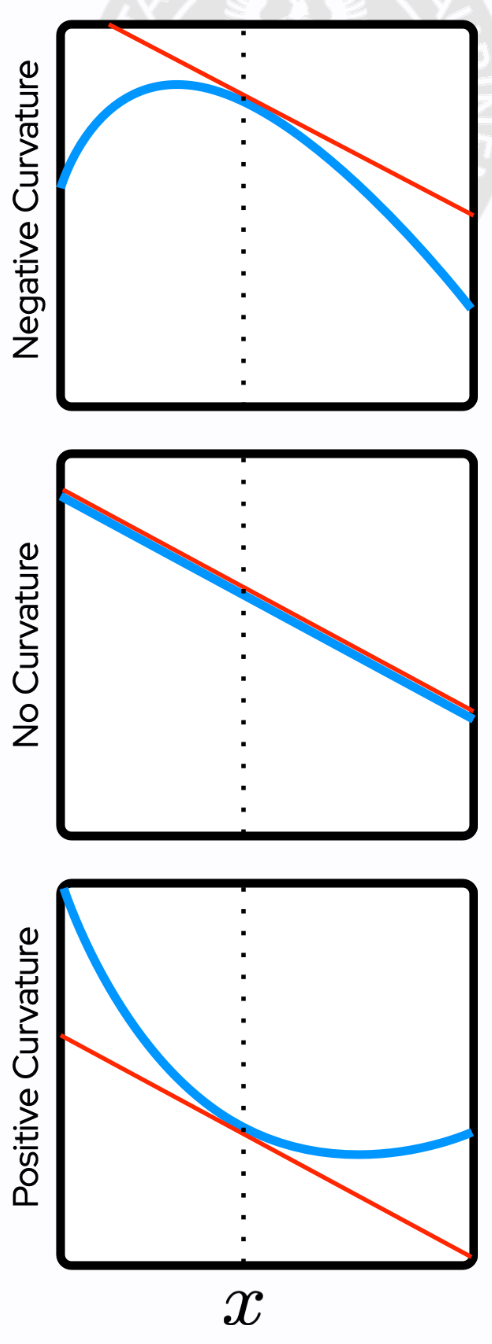
\includegraphics[scale=.55]{images/prerequisites/secondDerivative.png}
    \centering
\end{figure}


La matrice contenente tutte queste derivate parziali è chiamata \textbf{Hessiana} della funzione $f$.
\newline
\textbf{N.B.: }$H(f)=J(\nabla f)$.
\newpage

\paragraph{Proprietà della matrice Hessiana.}
\begin{itemize}
    \item in tutti in punti in cui le derivate seconde sono continue, gli operatori differenziali sono commutativi, cioè il loro ordine può essere scambiato:
        \begin{equation}
            \frac{\partial^2}{\partial x_i \partial x_j}f(x)=\frac{\partial^2}{\partial x_j \partial x_i}f(x)
        \end{equation}
        il che implica che \textbf{in quei punti la matrice Hessiana è simmetrica}.
    \item in maniera intuitiva, possiamo dire che, come la derivata seconda ci aiuta a capire se siamo in un punto di minimo o di massimo (indica la curvatura, quindi se la curvatura è verso l'alto siamo in un minimo, se è verso il basso siamo in un massimo), anche l'hessiano ci aiuta in questo senso. In particolare ci da questa informazione nel caso di \textbf{una funzione multi variata}. 


    In particolare, quando abbiamo che $\nabla f(x_0)=0$, \textbf{l'hessiano ci aiuta a capire se siamo in un minimo} (hessiano definito positivo\footnote{una matrice si definisce \textbf{positiva} quando $\forall z:z^TMz>0$}.) o \textbf{in un massimo} (hessiano definito negativo). Se l'hessiano non è ne definito positivo ne definito negativo (abbiamo almeno un autovalore che vale $0$):
    \begin{itemize}
        \item \textbf{siamo in un punto di sella}, se c'è almeno $1$ autovalore positivo e $1$ autovalore negativo;
        \item \textbf{il test non è conclusivo}, altrimenti.
    \end{itemize}
\end{itemize}
\newpage
\section{Probabilità}
La \textbf{probabilità} può essere vista come un'estensione della logica che tratta l'incertezza.


La \textbf{logica} fornisce una serie di regole formali per determinare quali proposizioni devono essere vere e quali false, data l'assunzione che un'altro set di proposizioni siano vere o false.


La \textbf{teoria delle probabilità} fornisce invece una serie di regole formali per determinare la \textbf{likelihood} di una proposizione data la likelihood di altre proposizioni.

Una \textbf{variabile casuale} è una variabile che può assumere randomicamente diversi valori. Possono essere \textbf{discrete} o \textbf{continue}.


Notazione:
\begin{itemize}
    \item variabili casuali sono indicate da lettere minuscole semplici come $x,t,\dots$;
    \item i valori assunti dalle variabili sono indicati da lettere minuscole in corsivo come $\textit{x},\textit{y},\dots$;
    \item il set di tutti i possibili valori assunti dalla variabile casuale $x$ è denotato da $\Omega_x$;
    \item a volte scriveremo $\textit{x}\in x$ per indicare $\textit{x}\in \Omega_x$;
    \item per valori che riguardano vettori e loro valori usere il grassetto quindi $\textbf{x,y}$ e $\textbf{\textit{x,y}}$.
\end{itemize}


\paragraph{Distribuzione di probabilità (Caso discreto)}
Sia data una \textbf{variabile discreta} $x={x_1,\dots,x_n}$. La \textbf{distribuzione di probabilità di una variabile discreta può essere indicata usando la probability mass function (PMF}. Normalmente essa è indicata con $\textit{P(x)}$.


La PMF \textbf{è un mapping che assegna ad ogni valore che può assumere la variabile casuale una probabilità}.
\begin{figure}[!h]
    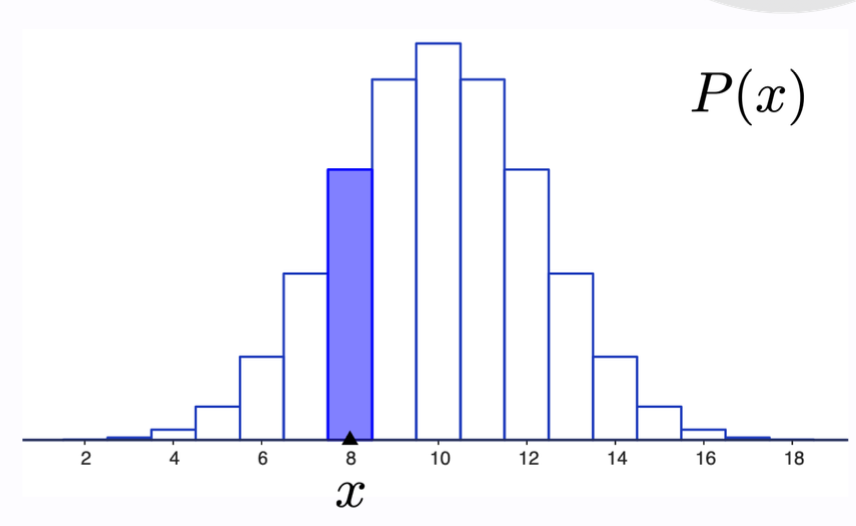
\includegraphics[scale=.5]{images/prerequisites/pmf.png}
    \centering
\end{figure}


\textbf{Notazione:} la probabilità che $\textit{P}(x=\textit{x})$ è denotata normalmente come $\textit{P}(x)$. La notazione $x\sim \textit{P}(x)$ è utilizzata per indicare che la variabile casuale $x$ segue la distribuzione descritta da $\textit{P}(x)$.



\textbf{Proprietà di una PMF:}
\begin{itemize}
    \item il dominio di $\textit{P}$ deve essere l'insieme di tutti i possibili stati di $x$;
    \item $\forall \textit{x}\in x:0\leq \textit{P}(\textit{x})\leq 1$;
    \item $\sum_{\textit{x}\in x}\textit{P}(\textit{x})=1$.
\end{itemize}
Altre proprietà utili sono:
\begin{itemize}
    \item $\textit{P}(\textit{S})=\sum_{\textit{x}\in \textit{S}}\textit{P}(\textit{x})$;
    \item $\textit{P}(\textit{$S_1$}\bigcup \textit{$S_2$})=\textit{P}(\textit{$S_1$})+\textit{P}(\textit{$S_2$})-\textit{P}(\textit{$S_1$}\bigcap \textit{$S_2$})$;
    \item $\textit{P}(\Omega \backslash \textit{S})=1-\textit{P}(\textit{S})$
\end{itemize}
con \textit{S},\textit{$S_1$},\textit{$S_2$} insiemi di possibili output; \textit{P}(\textit{S}) è una shortcut per $\textit{P}(x\in \textit{S})$ e $\Omega$ è l'insieme di tutti i possibili valori.


\paragraph{Distribuzione di probabilità (Caso continuo)}
In questo caso utilizziamo variabili \textbf{continue} e la distribuzion di probabilità non è più descrita dalla PMF ma dalla \textbf{probability density function (PDF)}.
\begin{figure}[!h]
    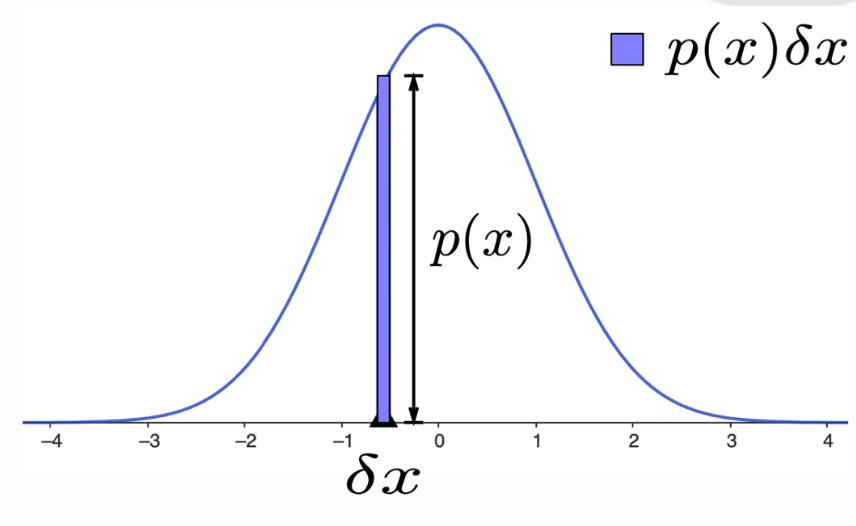
\includegraphics[scale=.5]{images/prerequisites/pdf.png}
    \centering
\end{figure}


La PDF è indicata con \textit{p} e deve soddisfare le seguenti proprietà:
\begin{itemize}
    \item il dominio di \textit{p} deve essere l'insieme di tutti i possibili stati di $\textbf{x}$;
    \item $\forall \textit{x}\in \textbf{x}:\textit{p}(\textit{x})\geq 0$, \textbf{notare che non richiediamo} $\textit{p}(\textit{x})\leq 1$;
    \item $\int \textit{p}(\textit{x})\textit{dx}=1$.
\end{itemize}

\subsection{Probabilità marginale}
A volte si conosce la distrivuzione di probabilità di un insieme di varibaili ma a noi interessa sapere la distribuzione di probabilità di un sottoineime di esse. In questo caso la distribuzione di probabilità è detta \textbf{distrubuzione marginale} di probabilità. 



Le probabilità marginali sono calcolate sommando tutti i valori delle variabili.


Per esempio, immaginiamo di avere 2 variabili casiali discrete $x$ e $y$ con una distribuzione congiunta $\textit{P}(x,y)$. La \textbf{distribuzione marginale} $\textit{P}(x)$ sarebbe:
\begin{equation}
    \forall \textit{x}\in x \textit{P}(\textit{x})=\sum_y\textit{P}(x=\textit{x},y=\textit{y});
\end{equation}
per le varabili continue:
\begin{equation}
    \textit{p}(\textit{x})=\int \textit{p}(\textit{x,y})\textit{dy}.
\end{equation}
\begin{figure}[!h]
    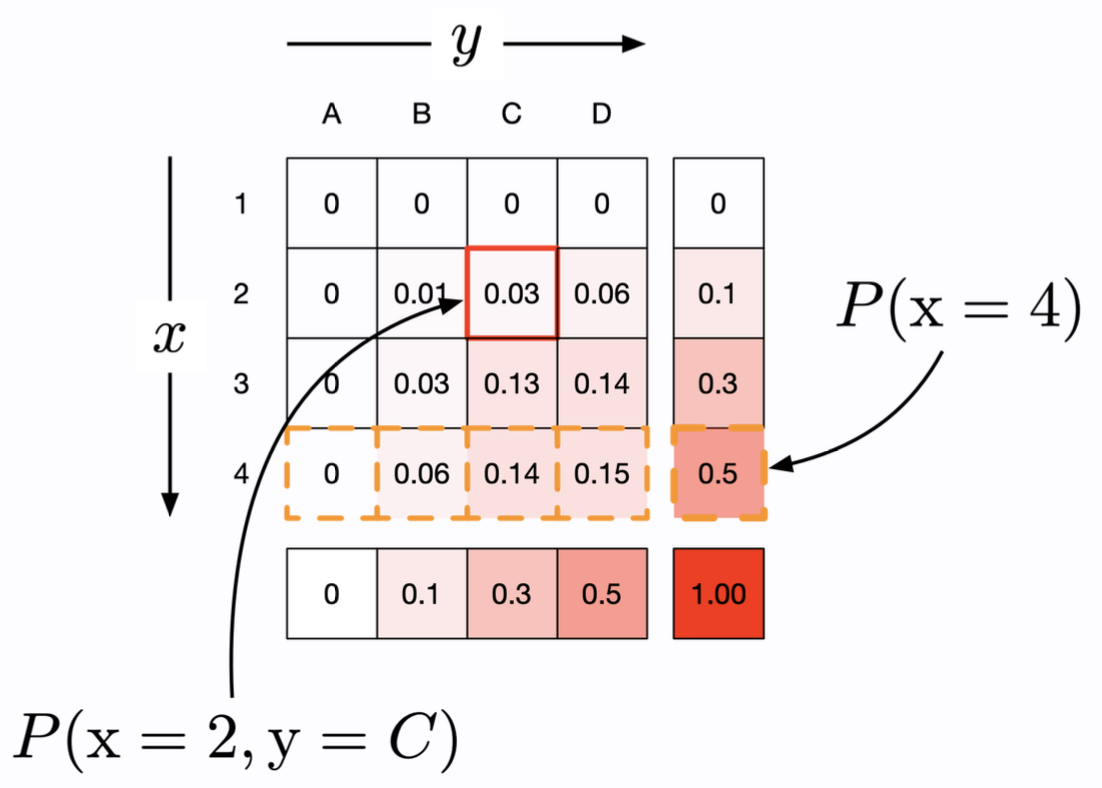
\includegraphics[scale=.5]{images/prerequisites/margProbability.png}
    \centering
\end{figure}
\newpage
\subsection{Probabilità condizionta}
In molti casi, siamo interessati alla probabilità di un evento dato un altro evento accaduto. Questa è la \textbf{probabilità condizionata}. La probabilità condizionata che $y=\textit{y}$ dato $x\textit{x}$ è indicata come
\begin{equation}
    \textit{P}(\text{y}=y|\text{x}=x).
\end{equation}
Può essere calcolata con la formula:
\begin{equation}
    P(\text{y}=y|\text{x}=x)=\frac{P(\text{y}=y,\text{x}=x)}{P(\text{x}=x)}.
\end{equation}
\begin{figure}[!h]
    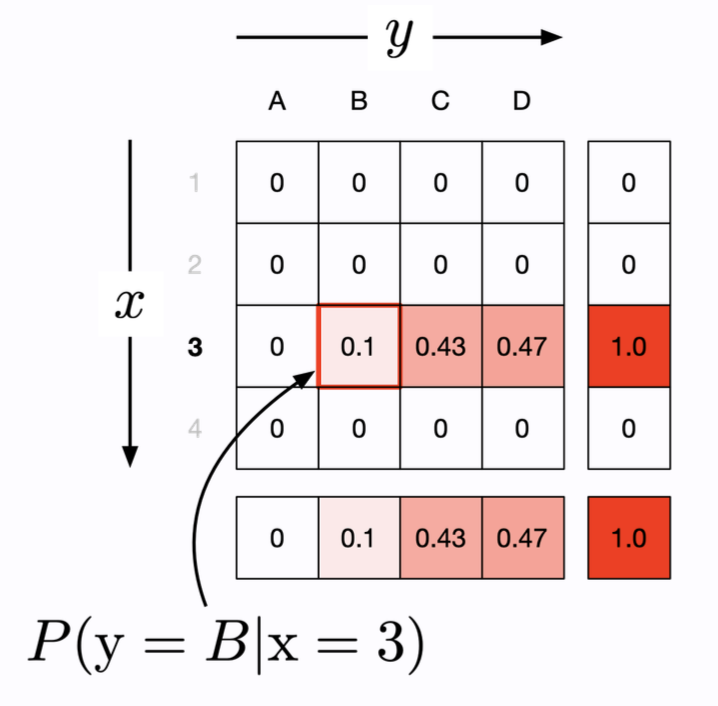
\includegraphics[scale=.5]{images/prerequisites/condProb.png}
    \centering
\end{figure}



La cosa interessante da notare è che questa \textbf{è una distrubizione completamente nuova su y}.


\subsection{Chain rule della probabilità condizionata}
Qualsiasi distribuzione di probabilità congiunta su più variabili casuali può essere decomposta in prodotti di distrivuzioni condizioni di una sola variabile:
\begin{equation}
    P(\text{x}^{(1)},\dots,\text{x}^{(n)})=P(\text{x}^{(1)})\prod^n_{i=2}P(\text{x}^{(i)}|\text{x}^{(1)},\dots,\text{x}^{(i-1)}).
\end{equation}
\textbf{Esempi}:
\begin{itemize}
    \item $P(\text{a}|\text{b,c})=\frac{P(\text{a,b,c})}{P(\text{b,c})} \Rightarrow P(\text{a,b,c})=P(\text{a$|$b,c})P(\text{b,c})$;
    \item similmente avremo che $P(\text{b,c})=P(\text{b$|$c})P(\text{c})$.
\end{itemize}
\subsection{Indipendenza}
Due variabili casuali x e y sono \textbf{indipendenti} (indicate con x$\perp$y) se \textbf{la loro distribuzione di probabilità può essere espressa come prodotto delle loro probabilità marginali}:
\begin{equation}
    \forall x\in \text{x},y\in \text{y}:p(\text{x}=x,\text{y}=y)=p(\text{x}=x)p(\text{y}=y).
\end{equation}
\textbf{Nota:}
\begin{equation}
    \text{x}\perp\text{y}\Longleftrightarrow \forall x\in \text{x},y\in \text{y}:p(x|y)=p(x) \wedge p(y|x)=p(y).
\end{equation}
Se è vero che le due variabili sono indipendenti valgono anche che:
\begin{itemize}
    \item $P(x|y)=P(x)$;
    \item $P(y|x)=P(y)$
\end{itemize}
il che è abbastanza intutivo, se le due variabili sono indipendenti le loro probabilità non hanno nessun impatto l'una sull'altra.
Inoltre, due variabili casuali x e y sono \textbf{condizionatamente indipenti} data una variabile casuale z (scriveremo x$\perp$y|z) se la distribuzione di probabilità condizionale su x e y fattorizza in questo modo per ogni valore di z:
\begin{equation}
    \forall x\in \text{x},y\in \text{y,z}\in \text{z}:p(\text{x}=x,\text{y}=y|\text{z}=z)=p(\text{x}=x|\text{z}=z)p(\text{y}=y|\text{z}=z).
\end{equation}

\subsection{Expectation (Valore atteso)}
Il \textbf{valore atteso} (spesso denotato da $\mu$) di una funzione $f(x)$ rispetto alla distribuzione di probabilità $P(\text{x})$ è la media o il valore medio che $f$ assume quando $x$ è tratto da $P$.



\textbf{Variabili discrete:}
\begin{equation}
    \mathbb{E}_{\text{x}\sim P}[f(x)]=\sum_xP(x)f(x).
\end{equation}
\textbf{Variabili continue:}
\begin{equation}
    \mathbb{E}_{\text{x}\sim p}[f(x)]=\int p(x)f(x)dx.
\end{equation}
\textbf{Nota:} il valore atteso è un \textbf{operatore lineare}:
\begin{equation}
    \mathbb{E}[\alpha f(x)+\beta g(x)]=\alpha \mathbb{E}[f(x)] + \beta \mathbb{E}[g(x)].
\end{equation}

\subsection{Varianza e Deviazione standard}
\paragraph{Varianza}
La varianza (spesso denotata con $\sigma^2$) restituisce la misure di \textbf{quando i valori di una funzione di una variabile casuale x variano rispetto al campionamento di diversi valori di x dalla sua distribuzione di probabilità}:
\begin{equation}
    \text{Var}[f(x)]=\mathbb{E}[(f(x)-\mathbb{E}[f(x)])^2].
\end{equation}
\textbf{Esempio:}
La varianza può anche essere calcolata come $\text{Var}[f(x)]=\mathbb{E}[f(x)^2]-\mathbb{E}[f(x)]^2$:
\begin{gather}
    \text{Var}[f(x)]=\mathbb{E}[(f(x)-\mathbb{E}[f(x)])^2]\\
    =\mathbb{E}[(f(x)^2-2f(x)\mathbb{E}[f(x)])+\mathbb{E}[f(x)])^2]\\
    =\mathbb{E}[f(x)^2]-2\mathbb{E}[f(x)\mathbb{E}[f(x)]])+\mathbb{E}[\mathbb{E}[f(x)]^2]\\
    =\mathbb{E}[f(x)^2]-2\mathbb{E}[f(x)]\mathbb{E}[f(x)]+\mathbb{E}[f(x)]^2\\
    =\mathbb{E}[f(x)^2]-\mathbb{E}[f(x)]^2.
    %%sistemare spaziatura
\end{gather}


\paragraph{Deviazione Standard.}
La \textbf{deviazione standard} (denotata da $\sigma$) è data dalla radice quadrata della varianza.


\textbf{Utile da sapere:} per una variabile descritta da una distribuzione normale, circa il 95\% dei punti cade in un range di $\mu \pm2\sigma$.



\paragraph{Covarianza.} La \textbf{covarianza} è una misura di quanto due variabili casuali siano relazionate l'una con l'altra:
\begin{gather}
    \text{Cov(x,y)}=\mathbb{E}_{x,y\sim P(\text{x,y})}[(x-\mathbb{E[\text{x}]})(y-\mathbb{E}[\text{y}])]\\
    =\mathbb{E}_{x,y\sim P(\text{x,y})}[(x-\mu_x)(y-\mu_y)]
\end{gather}
\begin{figure}[!h]
    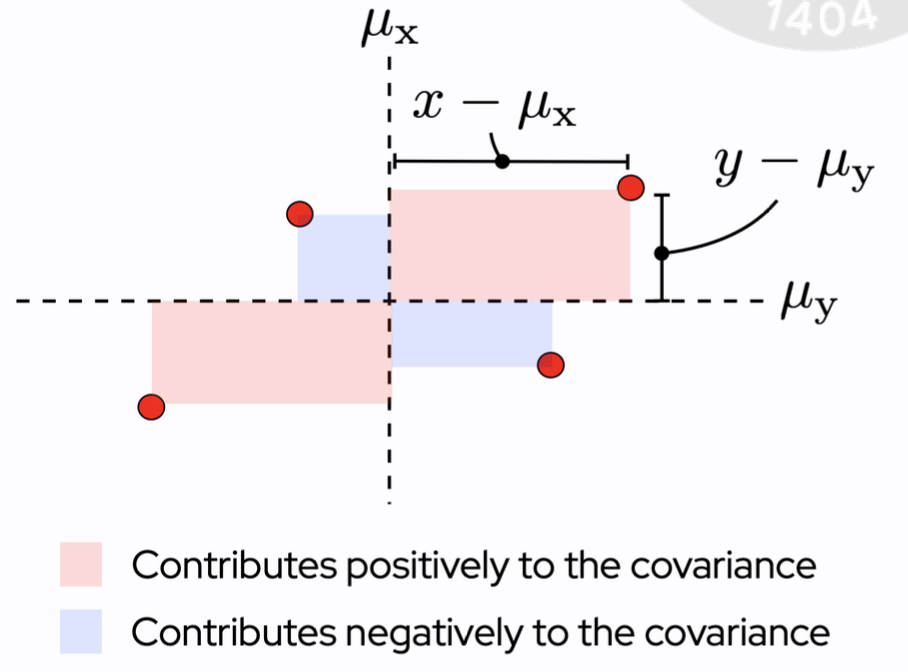
\includegraphics[scale=.5]{images/prerequisites/covariance.png}
    \centering
\end{figure}



L'idea è che, se $\mu_x$ e $\mu_y$ rappresentano gli assi (come in figura), prendendo un punto a caso (per esempio (x,y), punto rosso in alto a destra) mi posso chiedere in che maniera contribuisca al calcolo della covarianza. La risposta è che il contributo corrisponde all'area (rossa, nel caso di (x,y)) che sta sotto il rettangolo di cui il nostro punto rappresenta uno dei vertici. Quest'area contribuisce positivamente al calcolo se (x,y) sono entrambe maggiori delle rispettive medie, negativamente altrimenti.



\textbf{Nota:} la covarianza \textbf{è affetta dalla scala delle variabili}.



\paragraph{Correlazione.} La \textbf{correlation} risolve esattamente il problema appena descritto, cioè il fatto che la covarianza sia affetta dalla scala. Essa garantisce che la relazione tra le variabili sia misurata senza che sia influenzata dalle loro magnitudini invividuali:
\begin{equation}
    \text{Corr}(x,y)=\frac{\text{Cov}(x,y)}{\sigma_x\sigma_y}.
\end{equation}
Il risultato di questa formula restituisce un numero compreso in $[-1,1]$ ($+1$ le varabili assumono sempre gli stessi valori, $-1$ le variabili assumono sempre valori opposti) e una correlazione vicina a $\pm1$ indica una relazione forte tra le variavili mentre una correlazione vicina alle $0$ indica che le varibaili \textbf{potrebbero essere indipendenti}. 


\paragraph{Covarianza vs Dipendenza.} Le nozioni di \textbf{covarianza} e \textbf{dipendenza} sono correlate ma \textbf{sono concetti distinti}. Infatti:
\begin{itemize}
    \item due variabili che sono indipendenti hanno zero covarianza;
    %prima o poi scrivo questa dimostrazione, minuti 50 della lezione sulle probabilità

    
    \item due variabili che hanno covarianza diversa da zero sono dipendenti;
    \item due variabili possono avere covarianza pari a zero ed essere comunque dipendenti (come mostrato nella figura).
\end{itemize}
\begin{figure}[!h]
    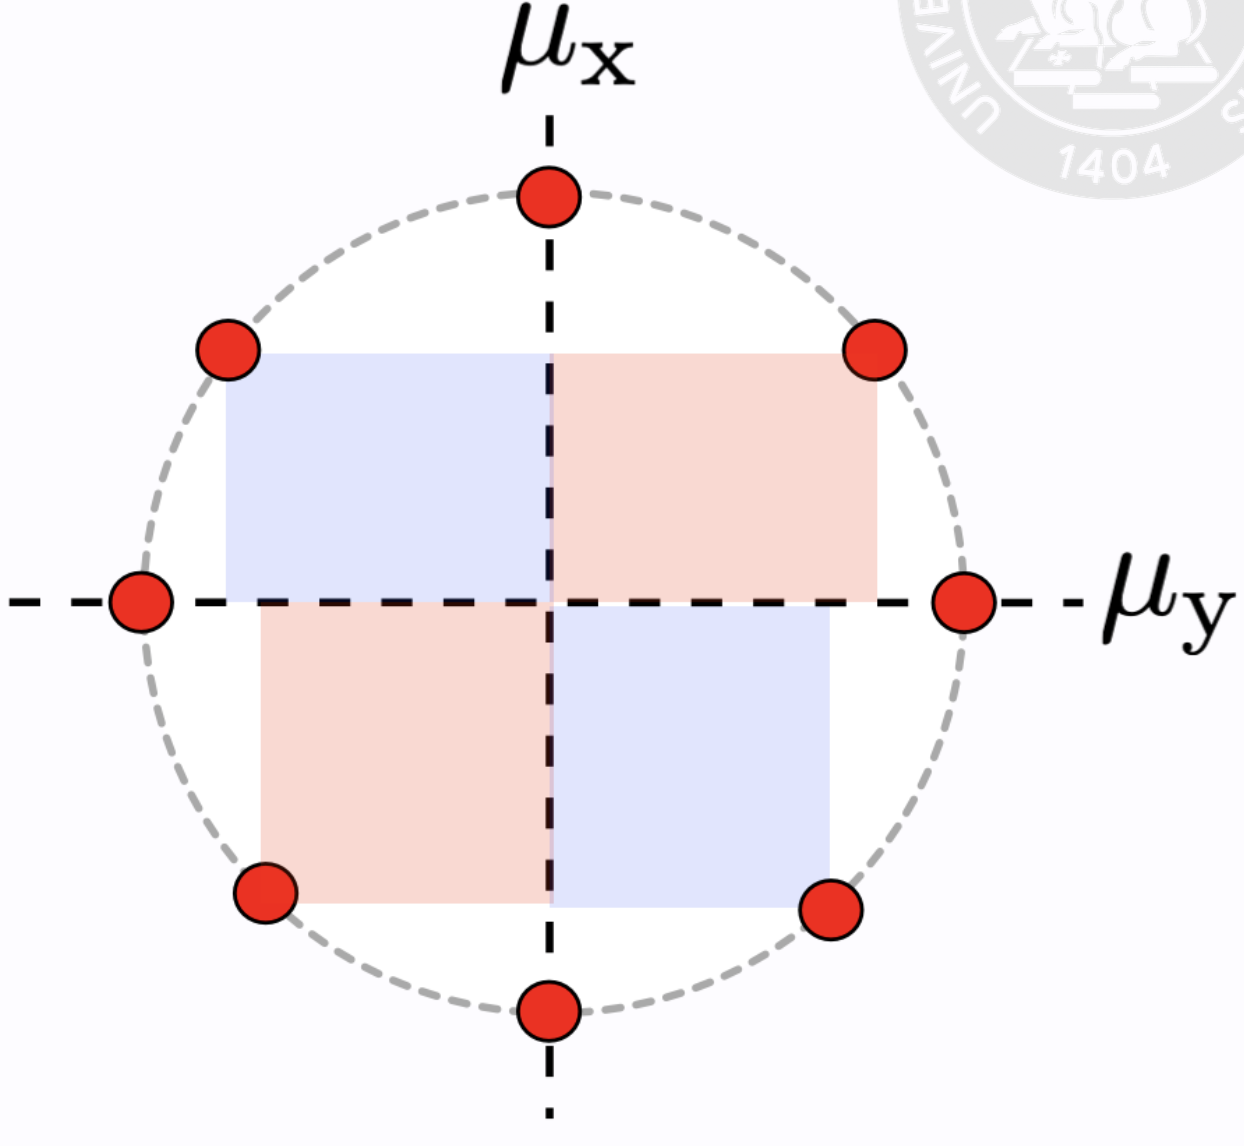
\includegraphics[scale=.25]{images/prerequisites/covVSdep.png}
    \centering
\end{figure}
\newpage

\subsection{Distribuzioni di Probabilità Comuni}
\paragraph{Bernoulli distribution.} Si tratta di una distribuzione di una singola variabile casuale \textbf{binaria} (semplicemente la distribuzione che modella il lancio di una moneta). E' controllata da un singolo parametro $\phi\in[0,1]$, il quale restituisce la probabilità che la variabile casuale abbia valore uguale ad $1$. Ha le seguenti proprietà:
\begin{itemize}
    \item $P(\text{x}=1)=\phi$;
    \item $P(\text{x}=0)=1-\phi$;
    \item $P(\text{x}=x)=\phi^x(1-\phi)^{1-x}$;
    \item $\mathbb{E}=\phi$;
    \item Var$(x)=\phi(1-\phi)$.
\end{itemize}


\paragraph{Multinoulli distribution.} E' un'estensione della distribuzione di Bernoulli a più di un risultato. La distribuzione \textbf{multinormale} o \textbf{categorica} tratta una singola variabile discreta com $k$ differenti stati, dove $k$ è finito.


E' parametizzata da un vettore \textbf{p}$\in[0,1]^k$, con \textbf{1}$^T$\textbf{p}$=1$ (che indica che gli elementi del vettore $p$ devono sommare ad $1$) dove $p_i$ restituisce la probabilità dell'$i-$esimo stato. 


Questo tipo di distribuzione è spesso usata per descrivere valori categorici, quindi normalmente non assumiamo che lo stato 1 ha valore numerico 1. Per questa ragione, \textbf{normalmente non abbiamo bisogno di calcolare l'expectation o la varianza} di variabili casuali di distribuzione multinormale.



\paragraph{Binomial distribution.} La distribuzione binomiale restituisce \textbf{la probabilità di osservare un dato numero di successi ripetendo l'esperimento di Bernoulli}. E' parametrizzata da:
\begin{itemize}
    \item $p$: la probabilità di successo dell'esperimento di Bernoulli;
    \item $N$: il numero totale di ripetizioni dell'esperimento di Bernoulli.
\end{itemize}
Se x$\sim$Bi($p,N$), allora:
\begin{gather}
    P(\text{x}=k)=\binom{N}{k}p^k(1-p)^{N-k}\\
    \mathbb{E}[\text{x}]=Np\\
    \text{Var[x]}=Np(1-p)
\end{gather}
\begin{figure}[!h]
    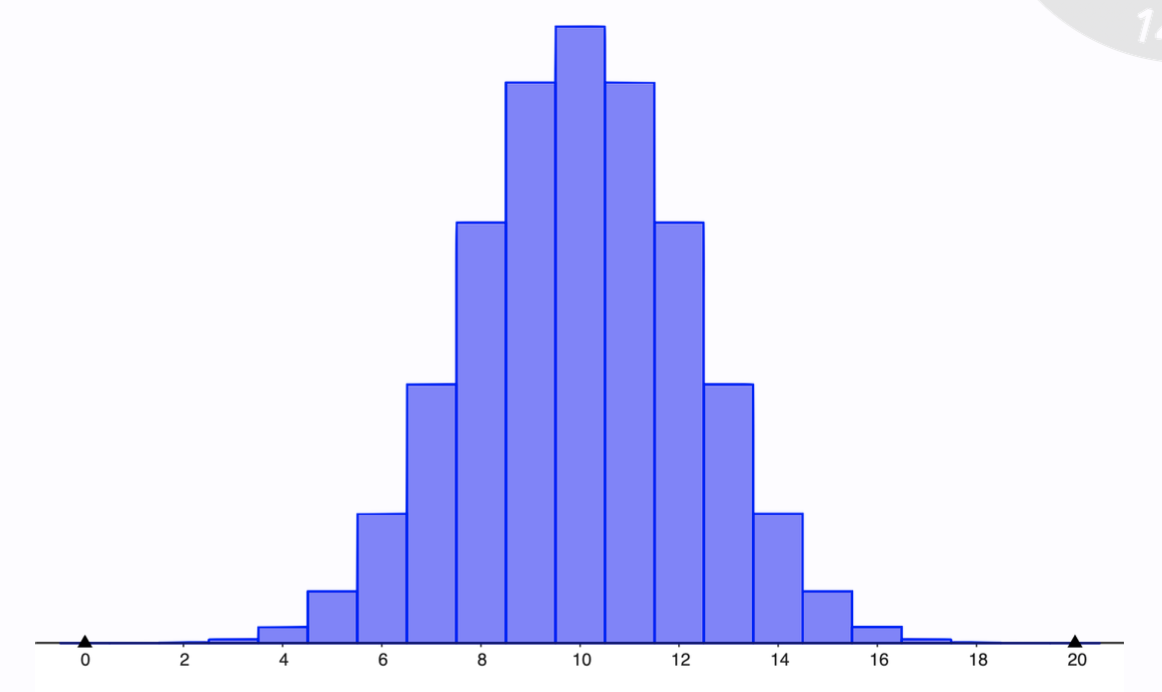
\includegraphics[scale=.5]{images/prerequisites/binomial.png}
    \centering
\end{figure}
\newpage
\paragraph{Gaussian distribution.} La distribuzione più utilizzata per i numeri reali è la \textbf{distribuzione normale}, anche detta \textbf{distribuzione Gaussiana}.


Una Gaussiana è parametrizzata da una media $\mu$ e da una varianza $\sigma^2$. Se x$\sim\mathcal{N}(\mu,\sigma^2)$, allora la PDF di x è data da:
\begin{equation}
    p(x)=\frac{1}{\sqrt{2\pi\sigma^2}}\text{exp}\Big( -\frac{(x-\mu)^2}{2\sigma^2} \Big).
\end{equation}
\begin{figure}[!h]
    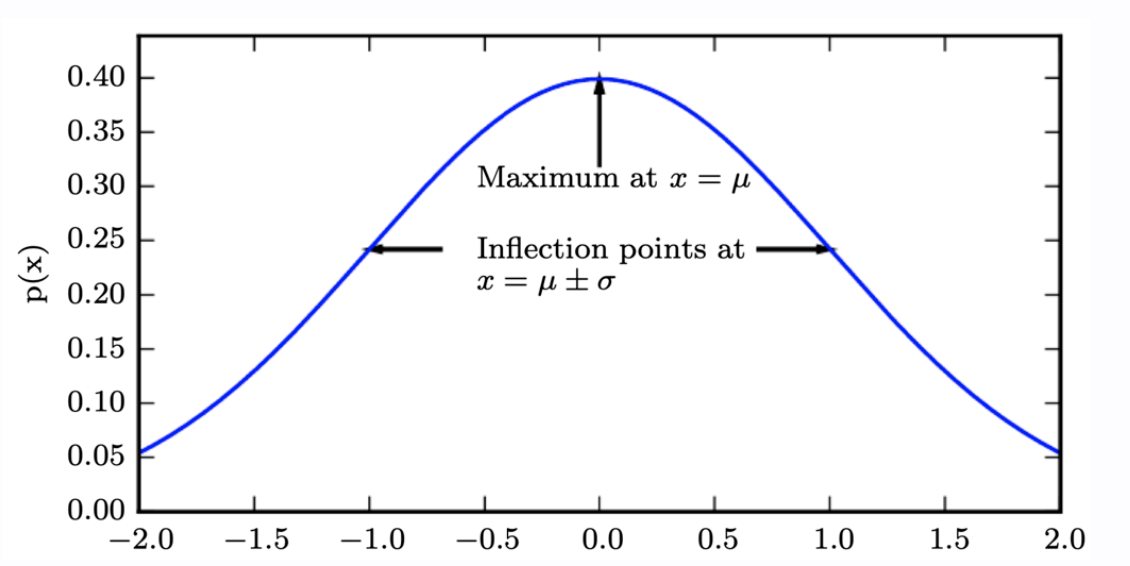
\includegraphics[scale=.5]{images/prerequisites/gaussian.png}
    \centering
\end{figure}



In realtà molte delle distribuzioni che vogliamo modellare sono molto vicine ad una distribuzione normale.
\paragraph{Teorema del limite centrale.} Sia $X_1,\dots,X_n$ una sequenza di variabili casueli indipendenti identicamente distribuite con media $\mu$ e varianza $\sigma^2$. La distribuzione della somma $S=\sum_{i=1}^nX_i$ tende ad una distribuzione normale $\mathcal{N}(n\mu,n\sigma^2)$ per $n$ che tende all'infinito. Anche la media $\frac{1}{n}S$ tende ad una distribuzione normale $\mathcal{N}(\mu,\frac{\sigma^2}{n})$ se $n$ tende all'infinito.
\newline
\newline
Tra tutte le possibili distribuzioni di probabilità con la stessa media e varianza, la distribuzione normale \textbf{codifica la massima quantità di incertezza} (cioè è la distribuzione che ha entropia massima). Ciò significa che se dobbiamo studiare un fenomeno di cui non abbiamo informazioni, l'ipotesi che si predilige, facendo meno assunzioni addizionali possibili riguardo il mondo esterno, è che segua la distribuzione normale.
\newline
\newline
La distribuzione normale si generalizza al caso multivariato $\mathbb{R}^n$:
\begin{equation}
    \mathcal{N}(\textbf{x;$\mu$,$\Sigma$)}=\frac{1}{\sqrt{(2\pi)^n\text{det}(\Sigma)}}\text{exp}\Big(-\frac{1}{2}(\textbf{x$-\mu$})^T\textbf{$\Sigma$}^{-1}(\textbf{x$-\mu$}) \Big)
\end{equation}
\begin{itemize}
    \item \textbf{$\mu$}: vettore che denota la media della distribuzione;
    \item \textbf{$\Sigma$}: la matrice di covarianza della distribuzione.
\end{itemize}
Leggiamo l'equazione:
\begin{itemize}
    \item $\frac{1}{\sqrt{(2\pi)^n\text{det}(\Sigma)}}$ è in realtà lo stesso fattore che troviamo nella Gaussiana ma che ha al posto di $\sigma^2$ il determinante della matrice di covarianza. Come nel caso precedente il fattore serve per riuscire a gestire meglio l'integrale;
    \item $(\textbf{x$-\mu$})^T\textbf{$\Sigma$}^{-1}(\textbf{x$-\mu$})$ non è altro che un'espressione quadratica, la cui formula generale è $z^TMz$.
\end{itemize}
Quindi nella sostanza è abbastanza simile alla formual della Gaussiana.
Le matrici di covarianza sono \textbf{simmetriche} e \textbf{semi-definite positive} e la loro diagonale principale contiene le varianze.


Se \textbf{$\Sigma=\sigma^2\mathbf{I}$}, la varianza è la stessa in ogni direzione: \textbf{la distribuzione è definita isotropica}.
\newpage
\paragraph{Exponential e Laplace distributions.} Nel contesto del deep learning, spesso vogliamo avere una distribuzione di probabilità con un picco in $x=0$. Per ottenere questo, possiamo usare la \textbf{distribuzione esponenziale}:
\begin{equation}
    p(x;\lambda)=\lambda\text{exp}(-\lambda x), x\geq0.
\end{equation}
\begin{figure}[!h]
    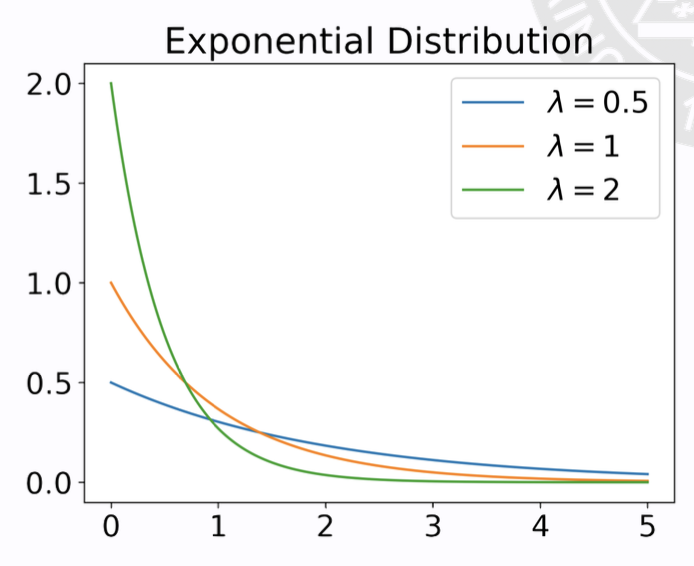
\includegraphics[scale=.7]{images/prerequisites/exp.png}
    \centering
\end{figure}
Il parametro $\lambda$ definisce quanto ripido è il picco.



Una distribuzione di probabilità correlata alla precedente, che ci permette di piazzare un picco di massa di probabilità in un punto arbitrario $\mu$ è la \textbf{distribuzione di Laplace}:
\begin{equation}
    \text{Laplace}(x;\mu,\gamma)=\frac{1}{2\gamma}\text{exp}\Big(-\frac{|x-\mu|}{\gamma} \Big)
\end{equation}
\begin{figure}[!h]
    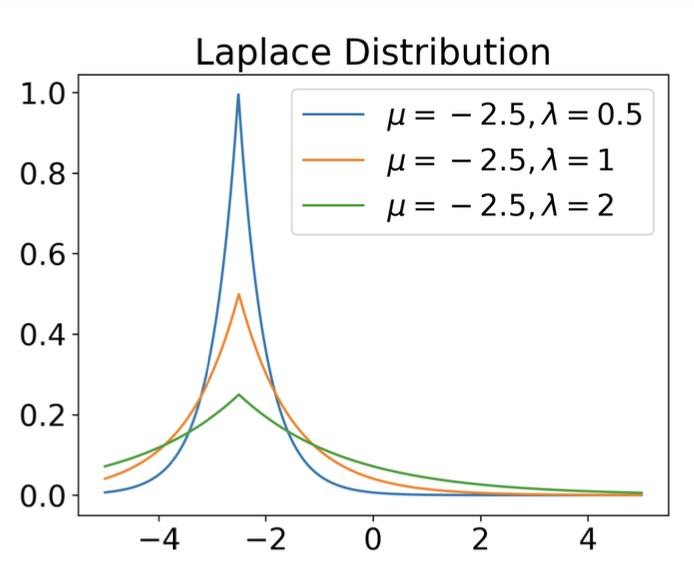
\includegraphics[scale=.7]{images/prerequisites/laplace.png}
    \centering
\end{figure}



In questo caso $\gamma$ ha lo stesso ruolo che aveva $\lambda$ nell'esponenziale mentre, come detto $\mu$ definisce in quale punto si trova il picco.
\newpage
\paragraph{Distribuzioni di tipo Mixture.} E' comune anche definire distribuzioni di probabilità a partire dalla combinazione di diverse semplici distribuzioni. Un modo comune di combinare distribuzioni è quello di costrure una \textbf{mixture distribution}:
\begin{equation}
    P(\text{x})=\sum_iP(\text{c}=i)P(\text{x|c}=i),
\end{equation}



dove $P(\text{c})$ è una distribuzione multinormale sui componenti della mistura.
\begin{figure}[!h]
    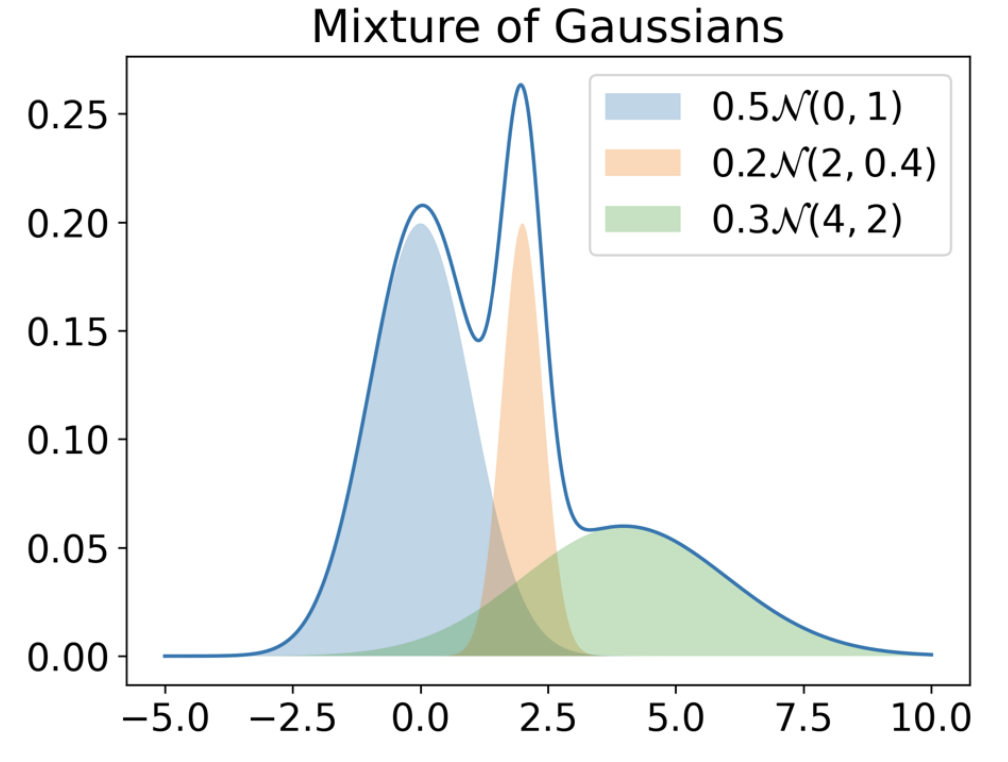
\includegraphics[scale=.6]{images/prerequisites/mixture.png}
    \centering
\end{figure}
\paragraph{Regola di Bayes.} Ci troviamo spesso in situazioni dove conosciamo $P(\text{y|x})$ e ci interessa conoscere $P(\text{x|y})$. Fortunatamente, se conosciamo anche $P(\text{x})$ e $P(\text{y})$, possiamo calcolare $P(\text{x|y})$ usando la \textbf{regola di Bayes}:
\begin{equation}
    P(\text{x$|$y})=\frac{P(\text{x})P(\text{y$|$x})}{P(\text{y})}.
\end{equation}




\paragraph{Variabili latenti.}
I mixture model ci permettono di accennare un concetto che avrà molta importanza in futuro: \textbf{le variabili latenti}.
\begin{figure}[!h]
    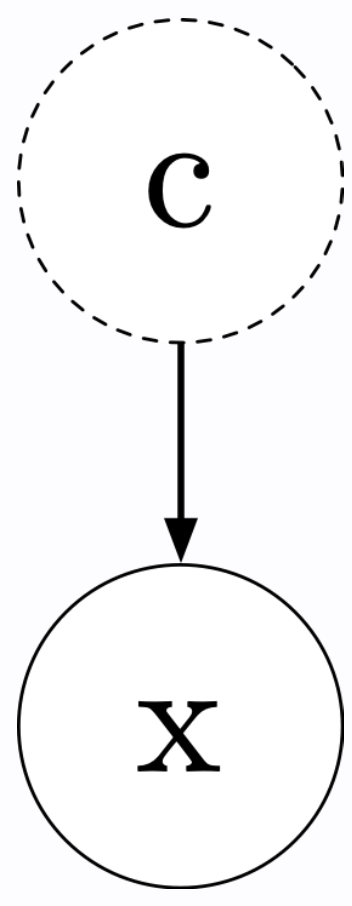
\includegraphics[scale=.3]{images/prerequisites/varLat.png}
    \centering
\end{figure}



Una variabile latente è una variabile casuale la quale \textbf{non può essere osservata direttamente} e che governa la distribuzione che stiamo osservando. Spesso assumere che ci sia una variabile latente ci permette di modellare e gestire meglio i problemi.
La variabile identità della componente \textbf{c} del mixture model ne fornisce un esempio.



Le variabili latenti potrebbero essere relazionate ad \textbf{x} attraverso la distribuzione congiunta, in questo caso, $P(\text{x,c})=P(\text{x$|$c})P(\text{c})$.
\newpage
\subsection{Proprietà utili delle funzioni comuni}
\paragraph{Sigmoid.} E' spesso usata per produrre il parametro $\phi$ della distribuzione di Bernoulli. E' denotata con $\sigma$ e definita come:
\begin{equation}
    \sigma(x)=\frac{1}{1+\exp(-x)}.
\end{equation}
\begin{figure}[!h]
    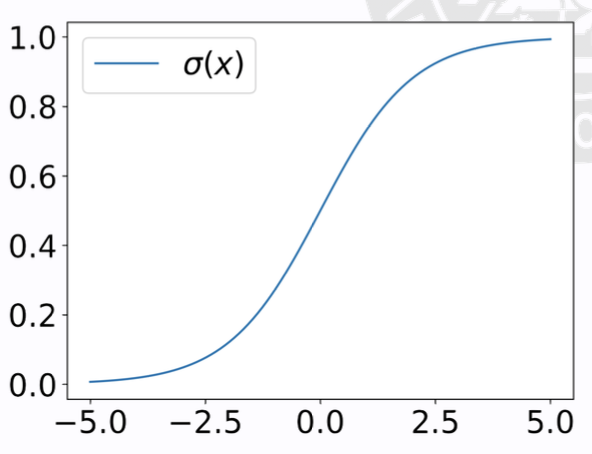
\includegraphics[scale=.7]{images/prerequisites/sigmoid.png}
    \centering
\end{figure}


\paragraph{Softplus.} Una versione \textbf{smooth} di $x^+=\max(0,x)$, è denotata con $\zeta$ e definita come:
\begin{equation}
    \zeta(x)=\log(1+\exp(x)).
\end{equation}
\begin{figure}[!h]
    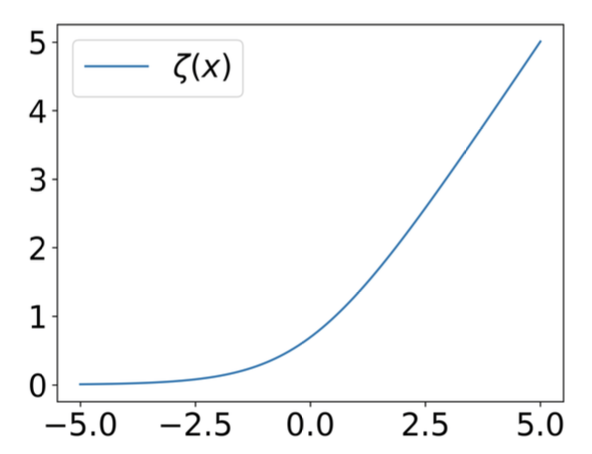
\includegraphics[scale=.7]{images/prerequisites/softplus.png}
    \centering
\end{figure}



\paragraph{Proprietà utili delle funzioni comuni.}
\begin{itemize}
    \item la sigmoide \textbf{si satura} per valori grandi (positivi e negativi) di $x$;
    \item $\sigma(x)=\frac{\exp(x)}{\exp(x)+\exp(0)}$;
    \item $\frac{d}{dx}\sigma(x)=\sigma(x)(1-\sigma(x))$;
    \item $1-\sigma(x)=\sigma(-x)$;
    \item $\log\sigma(x)=-\zeta(-x)$;
    \item $\frac{d}{dx}\zeta(x)=\sigma(x)$;
    \item $\forall x\in(0,1):\sigma^{-1}(x)=\log(\frac{x}{1-x})$;
    \item $\forall x>0:\zeta^{-1}(x)=\log(\exp(x)-1)$;
    \item $\zeta(x)=\int^x_{-\infty}\sigma(y)dy$;
    \item $\zeta(x)-\zeta(-x)=x$.
\end{itemize}
\newpage
\subsection{Measure Theory}
Una corretta comprensione formale delle variabili casuali continue e della probability density function richiede uno sviluppo della teoria delle probabilità attravero un ramo della matematica conosciuto come \textbf{measure theory} o teoria della misura.
\newline
\newline
Senza di essa, potremmo ritrovarci in situationi paradossali come:



\textit{è possibile costruire due insiemi} $S_1$ \textit{e} $S_2$, \textit{con} $S_1\cap S_2=\emptyset$ \textit{tali che} $p(x\in S_1)+p(x\in S_2)>1$.
\newline
\newline
Questi paradossi spesso riguardano la costruzione di insiemi \textit{molto esotici}, come insiemi frattali o che derivano da trasformazioni di numeri razionali, ma la possibilità esiste.
\newline
\newline
Uno dei contributi chiave di questa è il fatto che fornisca un framework per caratterizzare insiemi in cui le probabilità possono essere calcolate in maniera consistente, evitando paradossi.


La measure theory fornisce un modo rigoroso per descrivere che \textbf{un insieme di punti è trascurabilmente piccolo}. In questo caso diremo che l'insieme ha \textbf{measure zero}, o misura zero. 
\newline
\textbf{Esempio:}
\textit{Una linea in $\mathbb{R}^2$ ha measure zero}.
\newline
\newline
Qualsiasi \textbf{unione di insiemi numerabili} che abbiano measure zero ha anch'essa measure zero (quindi l'insieme di tutti i numeri razionali ha measure zero).


Quando una proprietà vale in tutto lo spazio tranne che per un punto in un insieme di misura zero, diremo che quella proprietà vale \textbf{quasi ovunque}.



\paragraph{Dettagli tecnici delle variabili continue.} Trattiamo ora le variabili casuali continue che sono \textbf{funzioni deterministici di altre variabili}. 



Supponiamo di avere due variabili casuali, \textbf{x} e \textbf{y}, tali che \textbf{$y$}=g(\textbf{$x$}), dove $g$ è una trasformazione differenziabile, invertibile e continua.


Sfortunatamente: $p_\text{y}(y)\neq p_\text{x}(g^{-1}(y))$.
\newline
\newline
Sia y$=\frac{\text{x}}{2}$ e x$\sim U(0,1)$. In questo caso abbiamo:
\begin{itemize}
    \item $y=g(x)=\frac{x}{2}$;
    \item $x=g^{-1}(y)=2y$.
\end{itemize}
\begin{figure}[!h]
    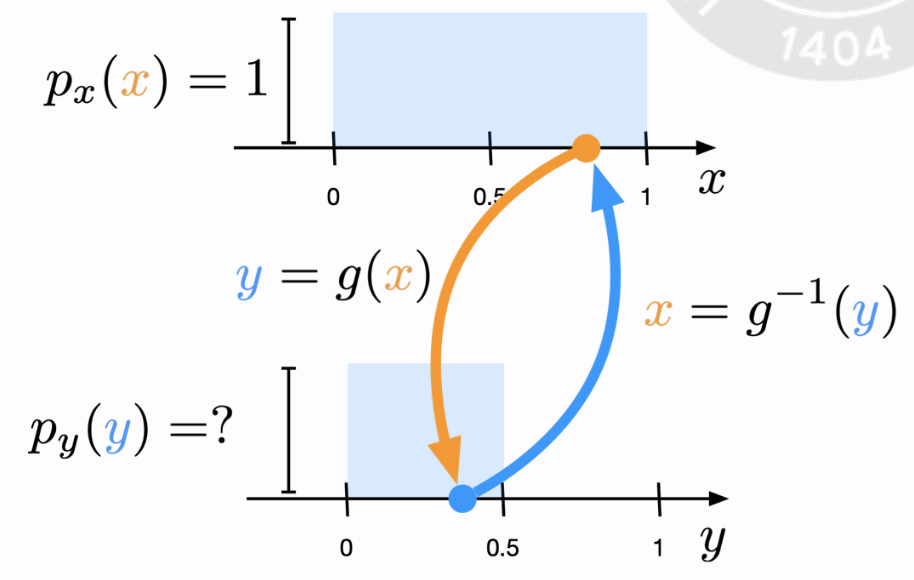
\includegraphics[scale=.5]{images/prerequisites/ex01.png}
    \centering
\end{figure}



Ci aspetteremo che $p_y(y)=p_x(2y)$, ma non è questo il caso. Infatti, se così fosse, $p_y(y)$ sarebbe uguale a zero dapperttutto ad eccezione dell'intervallo $[0,\frac{1}{2}]$ dove sarebbe $1$. Invece:
\begin{equation}
    \int_{-\infty}^\infty p_y(y)dy=\int_0^{0.5}1dy=x\Big|^{0.5}_0=0.5-0=0-5
\end{equation}


Il problema con questo approccio è che fallisce nel tenere conto della distorsione dello spazio introdotta dalla funzione $g$.



La probabilità che $x$ si trovi in una regione infinitesimamente piccola con volume $\delta x$ è data da $p(x)\delta x$.
\begin{figure}[!h]
    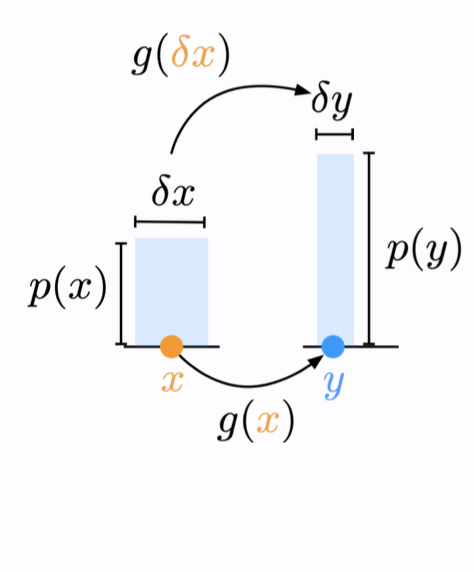
\includegraphics[scale=.7]{images/prerequisites/ex02.png}
    \centering
\end{figure}



Siccome $g$ può espandere o contrarre lo spa<io, il volume infinitesimale che circonda $x$ nello spazio $x$ potrebbe avere un volume differente nello spazio $y$.



Per correggere il problema abbiamo bisogno di preservare la proprietà:
\begin{equation}
    |p_y(g(x))dy|=|p_x(x)dx|
\end{equation}
che porta a:
\begin{equation}
    p_y(g(x))|dy|=p_x(x)|dx| \Rightarrow p_x(x)=p_y(g(x))\Big| \frac{d}{dx}g(x) \Big|
\end{equation}
o, equivalentemente:
\begin{equation}
    p_y(y)|dy|=p_x(g^{-1}(y))|dx| \Rightarrow p_y(y)=p_x(g^{-1}(y))\Big| \frac{d}{dy}g(y) \Big|.
\end{equation}



Nel nostro esempio:
\begin{equation}
    p_y(y)=p_x(g^{-1}(y))\Big| \frac{\partial g^{-1}(y)}{\partial y} \Big|=p_x(2y)\Big| \frac{d}{dy}2y\Big|=1\cdot2=2
\end{equation}
e
\begin{equation}
    \int_0^{0.5}p_y(y)dy=\int_0^{0.5}2dy=1.
\end{equation}
In \textbf{dimensioni maggiori} $g:\mathbb{R}^m\rightarrow\mathbb{R}^n$, la derivata si generalizza alla matrice jacobiana e il valore assoluto al valore assoluto del determinante:
\begin{equation}
    p_x(x)=p_y(g(x))|\text{det}(J)|
\end{equation}
dove la jacobiana $J$ è tale è $J_{ij}=\frac{\partial g(x)_i}{\partial x_j}$.







\newpage
\section{Information theory}
L'\textbf{information theory} è una branca della matematica applicata che ruota attorno alla quantificazione della quantità di informazioni presenti in un segnale.


In questo corso, useremo alcune delle idee chiave della information theory per \textbf{caratterizzare distribuzioni di probabilità} o \textbf{misurare la similarità tra distribuzioni di probabilità}.


\subsection{Quantificare l'informazione}
L'intuizione base dietro l'information theory è il fatto che la quantità di informazione trasportata da un messaggio dipende da quanto esso sia probabile: sapere che un \textbf{evento improbabile} sia accaduto \textbf{è più informativo} di sapere che un evento probabile sia accaduto.


\textbf{Esempio:}



\textit{Sapere che oggi ha piovuto nel deserto del Sahara è più informativo di saoere che oggi ha piovuto a Londra.}
\newline
\newline
Volendo formalizzare questa intuizione:
\begin{itemize}
    \item un evento con probabilità del $100\%$ è \textbf{assolutamente non sorprendente e non produce informazioni};
    \item \textbf{meno l'evento è probabile} più è sorprendente e \textbf{più produce informazioni};
    \item \textbf{eventi indipendenti dovrebbero produrre informazioni aggiuntive}. Per esempio, scoprire che una moneta lanciata ha dato testa due volte dovrebbe fornire il doppio delle informazioni rispetto a scoprire che una moneta lanciata ha dato testa una volta.
\end{itemize}
\newpage
\paragraph{Misura dell'entropia di Shannon.} Possiamo quantificare l'incertezza di un evento utilizzando il concetto di \textit{self-information measure}:
\begin{equation}
    I(x)=-\log P(x)
\end{equation}


la quale equazione gode delle proprietà descritte precedentemente:
\begin{itemize}
    \item se un evento ha probabilità del $100\%$ allora $\log 1=0$ e non produce informazioni;
    \item più la probabilità dell'evento si abbassa, più produce informazione. Infatti il logaritmo di un numero vicino allo $0$ tende a $-\infty$.
\end{itemize}
\textbf{L'entropia di Shannon} è definita come il \textbf{valore atteso della self-information measure}, in maniera più formale cattura la quantità media di "informazioni" su tutti i possibili risultati di una variabile casuale:
\begin{equation}
    H(\text{x})=E_{\text{x}\sim P}[I(\text{x})]=-\sum_xP(x)[\log(P(x))].
\end{equation}
Il \textbf{Shannon's Source Coding Theorem} afferma che $H(\text{x})$ fornisce un confine inferiore per la lunghezza media della parole da utilizzare per ottenere una codifica ottimale di tutti i possibili valori di x.
\begin{figure}[!h]
    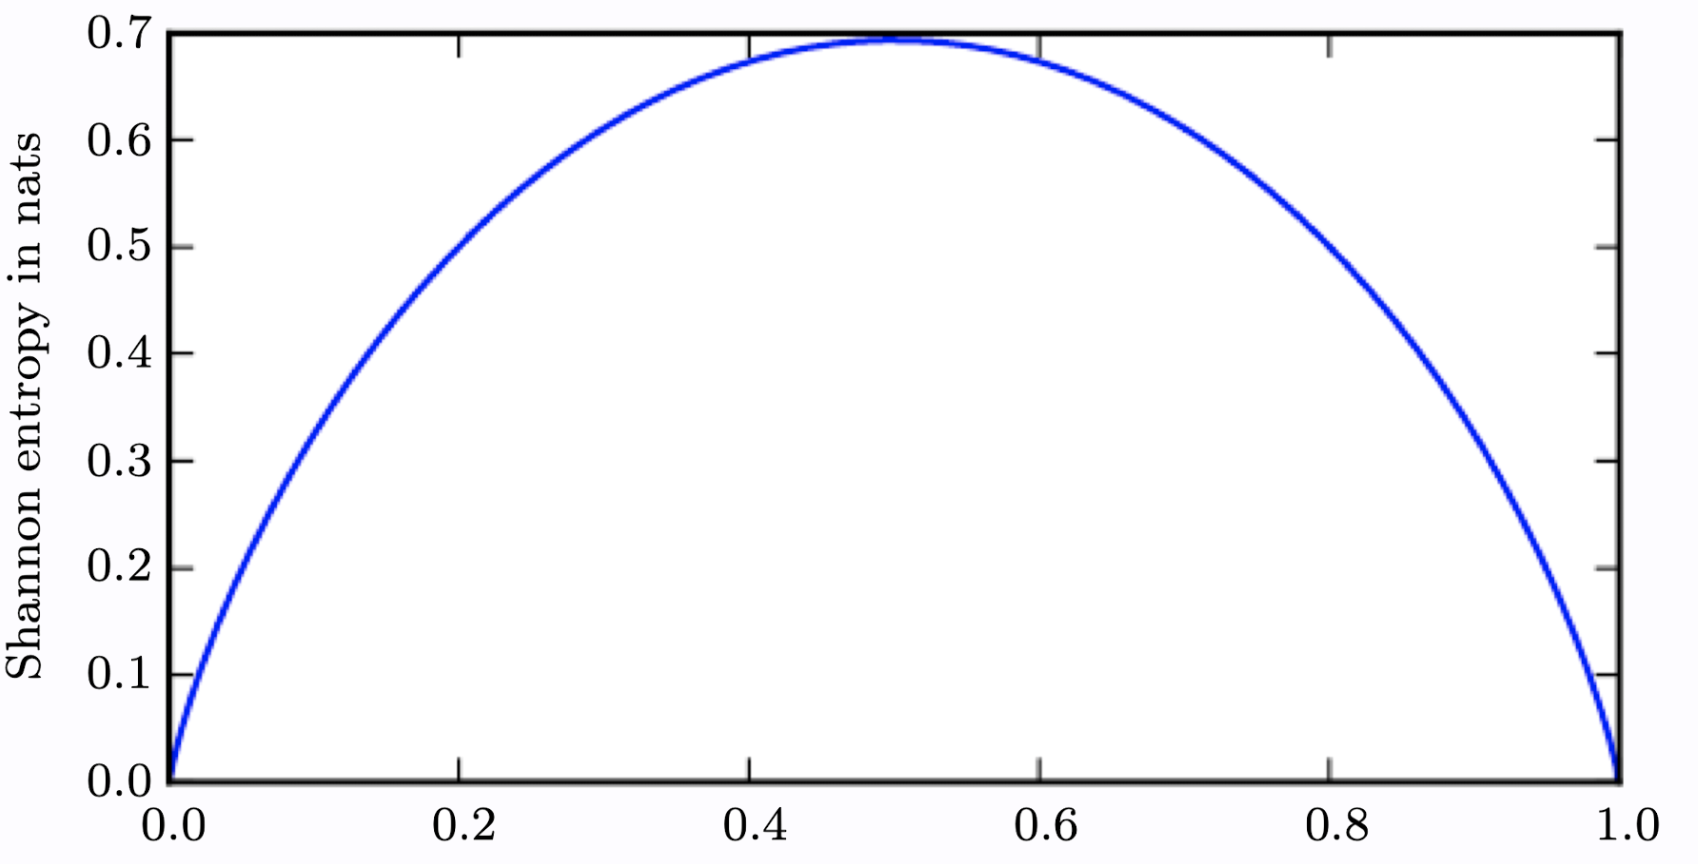
\includegraphics[scale=.5]{images/prerequisites/shannon.png}
    \caption{L'entropia di una variabile casuale \textbf{x}$\sim$\textbf{Bernoulli}($\phi$) al variare di $\phi$ tra $0$ e $1$.}
    \centering
\end{figure}


\paragraph{La divergenza Kullback-Leibler(KL).} Se abbiamo due distribuzioni separate $P(\text{x})$ e $Q(\text{x})$ della stessa variabile x, possiamo misurare quanto siano differenti l'una dall'altra utilizzando la \textbf{Kullback-Leibler divergence}:
\begin{equation}
    D_{\text{KL}}(P\|Q)=E_{\text{x}\sim P}\Big[ \log\frac{P(x)}{Q(x)} \Big]=E_{\text{x}\sim P}[\log P(x)-\log Q(x)].
\end{equation}
Nel caso di variabili discrete, rappresenta la \textbf{quantità extra di informazioni} di cui si necessita per inviare un messaggio contenente simboli estratti dalla distribuzione di probabilità $P$, quando usiamo codice il cui design è pensato per minimizzare la lunghezza di messaggi estratti dalla distribuzione di probabilità $Q$.



\paragraph{Proprietà della KL divergence.}
\begin{itemize}
    \item la KL divergence è sempre \textbf{non negativa};
    \item la KL divergence è $0\Longleftrightarrow P$ e $Q$ sono la stessa distribuzione (o sono ugali \textit{quasi in ogni punto} nel caso di variabili continue);
    \item la KL divergence \textbf{non è una misura di distanza}: una distanza dovrebbe essere simmetrica e soddisfare la disuguaglianza triangola, ma la KL divergence non o fa.
\end{itemize}
Quest'ultimo punto, in particolare il fatto che non sia simmetrica, ha importanti conseguenza quando bisogna minimizzare la \textbf{distanza} tra le due distribuzioni $P$ e $Q$.



\paragraph{Minimizzare la KL divergence.} Minimizzare $D_{\text{KL}}(p\|q)$ può essere molto diverso da minimizzare $D_{\text{KL}}(q\|p)$.
Assumiamo che:
\begin{itemize}
    \item $p$ sia una mistura di due Gaussiane con 2 diverse mode;
    \item $q$ sia una singola Gaussiana che vogliamo \textbf{ottimizzare} in modo che matchi $p$ nel modo migliore possigile.
\end{itemize}
\begin{equation}
     D_{\text{KL}}(p\|q)=E_{\text{x}\sim p}\Big[ \log\frac{p(x)}{q(x)}\Big].
\end{equation}
\begin{figure}[!h]
    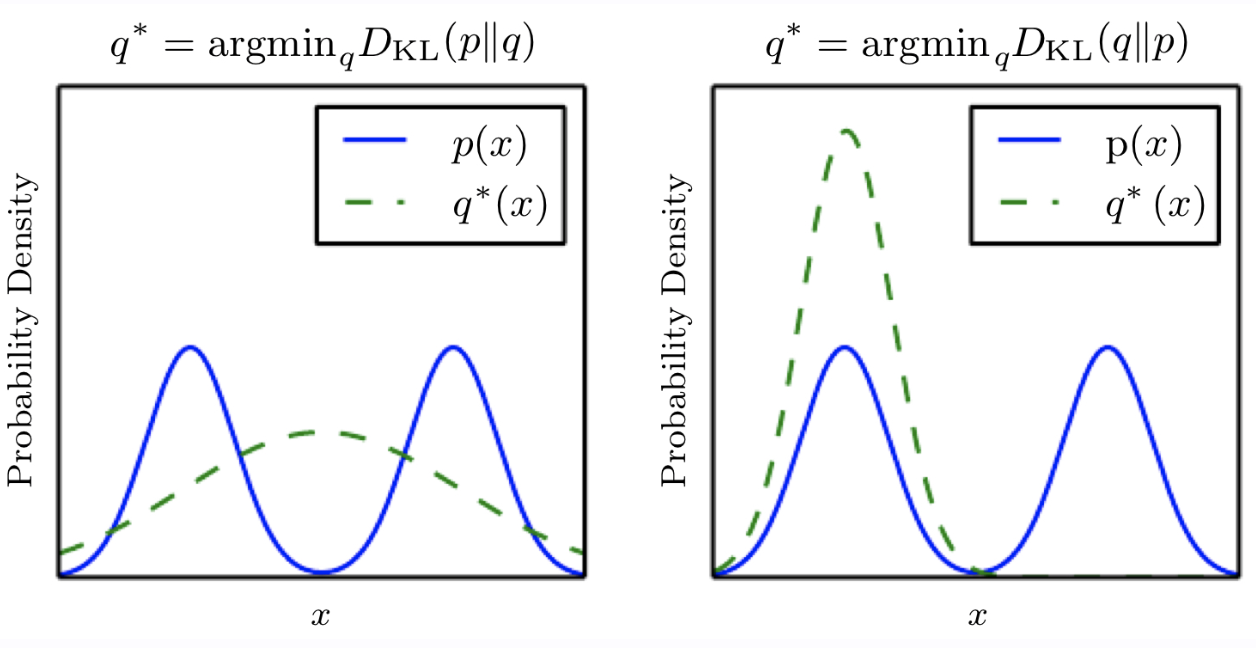
\includegraphics[scale=.6]{images/prerequisites/kl01.png}
    \centering
\end{figure}
\begin{equation}
     D_{\text{KL}}(q\|p)=E_{\text{x}\sim q}\Big[ \log\frac{q(x)}{p(x)}\Big].
\end{equation}
\newpage
\begin{equation}
    \min_q[D_{\text{KL}}(p\|q)]=\min_q\Big[ \mathbb{E}_{\text{x}\sim p}\Big[\log\frac{p(x)}{q(x)} \Big]\Big]
\end{equation}
\begin{figure}[!h]
    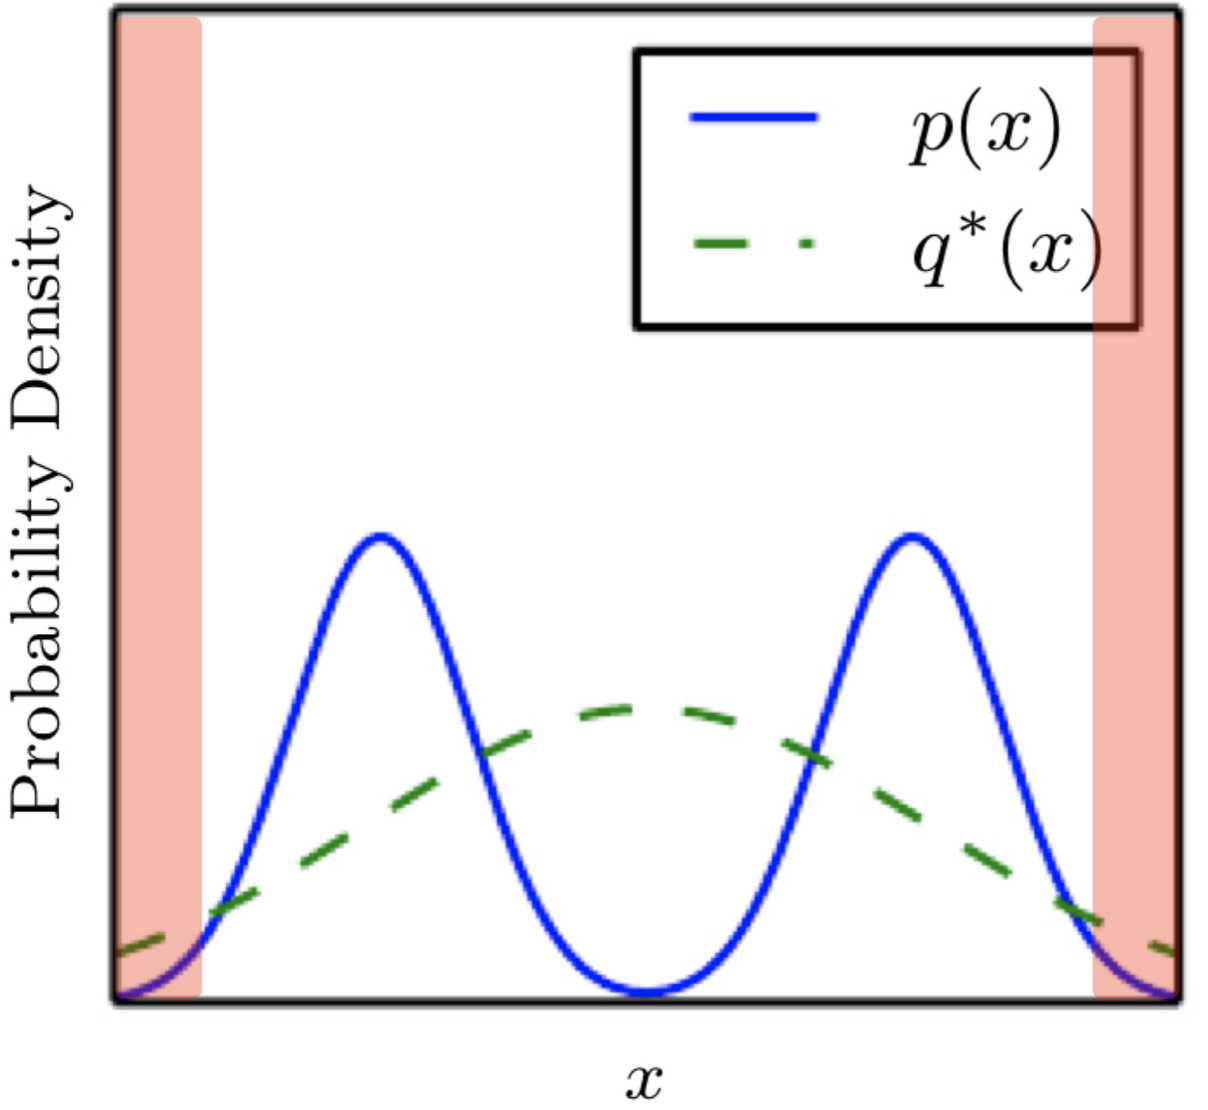
\includegraphics[scale=.5]{images/prerequisites/kl02.png}
    \centering
\end{figure}
\begin{equation}
    \min_q[D_{\text{KL}}(q\|p)]=\min_q\Big[ \mathbb{E}_{\text{x}\sim q}\Big[\log\frac{q(x)}{p(x)} \Big]\Big]
\end{equation}
\begin{figure}[!h]
    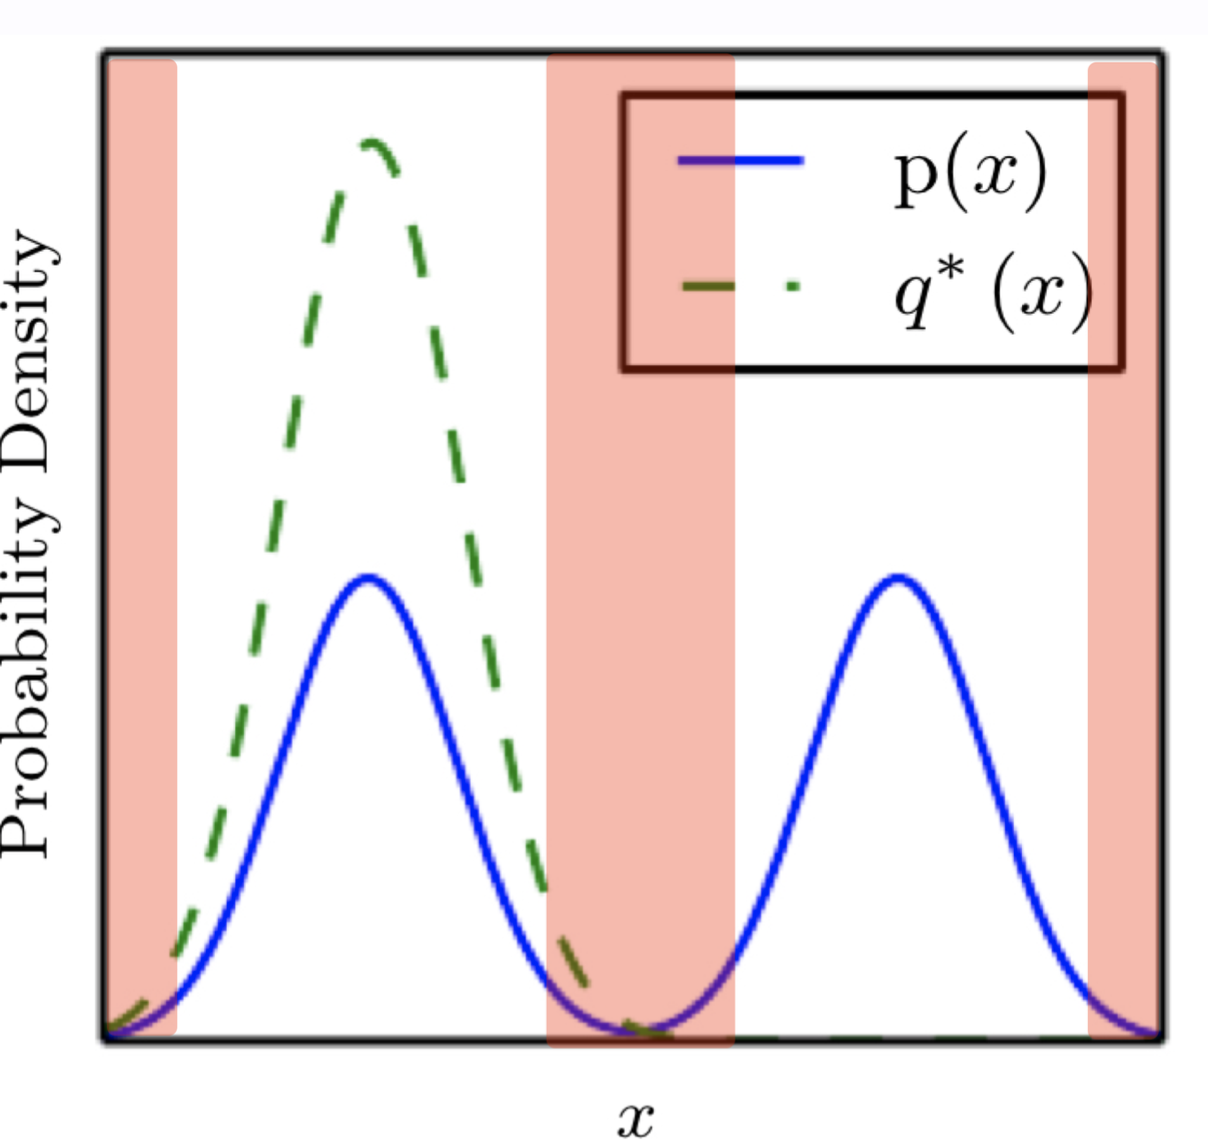
\includegraphics[scale=.5]{images/prerequisites/kl03.png}
    \centering
\end{figure}
\newpage
\paragraph{Cross Entropy.} Una quantità che è strettamente correlata alla KL divergence è la \textbf{cross-entropy}:
\begin{equation}
    H(P,Q)=H(P)+D_{\text{KL}}(P\|Q)=-E_{\text{x}\sim P}[\log Q(x)]
\end{equation}
cioè la cross entropy è \textbf{il numero medio di bit necessari per codicare un messaggio del codice $Q$ con un codice pensato per $P$}.


\textbf{Note:}
\begin{itemize}
    \item è simile a $D_{\text{KL}}(P\|Q)=E_{\text{x}\sim P}[\log P(x)-\log Q(x)]$:
    \begin{itemize}
        \item expressioni simili ma manca il termine $\log Q(x)$;
        \item concettualmente differente è il fatto che $D_{\text{KL}}$ misuri il numero di bit extra previsto mentre $H$ misuri il numero totale di bit.
    \end{itemize}
    \item minimizzare $H(P,Q)$ rispetto a $Q$ è la stessa cosa di minimizzare $D_{\text{KL}}(P\|Q)$. 
\end{itemize}    
    
Il motivo si vede bene guardando il fattore $H(P)+D_{\text{KL}}(P\|Q)$; infatti quando minimizziamo $P$ e $Q$ lo facciamo rispetto alla distribuzione $Q$, in questo fattore si vede bene che c'è un termine, $H(P)$, che non dipende dalla distribuzione $Q$, e il secondo termine, che è esattamente la KL, che invece dipende da $Q$. Perciò sostanzialmente stiamo andando a minimizzare la KL anche quando minimizziamo la cross-entropy. \textbf{Il punto è che spesso è più semplice minimizzare la cross-entropy perchè ha una forma più semplice rispetto alla KL.}

\newpage

\subsection{Modelli grafici (modelli probabilistici strutturati)}
Spesso le distribuzioni di probabilità possono essere divise in molti fattori. Per esempio, assumiamo che un variabile casuale $a$ influenzi il valore di un'altra variabile $b$ e che questa a sua volta influenzi $c$, ma sono indipendeti l'una rispetto all'altra. Possimo rappresentare l'intera distribuzione come segue:
\begin{equation}
    p(a,b,c)=p(a)p(b|a)p(c|b).
\end{equation}
Questi tipi di fattorizzazione possono \textbf{ridurre enormemente il numero di parametri} necessari per descrivere una distribuzione.
\newline
\newline
\textbf{Esempio:}


Assumiamo che $a,b,c$ assumano tutte valori in $\{1,2,3,4,5\}$. Per descrivere completamente le probabilità coinvolte dovremmo specificare $5^3=125$ valori di probabilità.


Se la distribuzione fattorizza come sopra abbiamo bisogno solo di:
\begin{itemize}
    \item $5$ parametri per descrivere $p(a)$;
    \item $25$ parametri per descrivere $p(b|a)$;
    \item $25$ parametri per descrivere $p(c|b)$.
\end{itemize}

\paragraph{Modelli grafici.} Le fattorizzazioni sulle distribuzioni possono essere visivamente descritti usando i grafi.
\paragraph{Modelli diretti.} Utilizzano grafi con archi diretti. Rappresentano le fattorizzazioni in distribuzioni di probabilità condizionate:
\begin{itemize}
    \item un fattore per ogni variabile casuale x$_i$;
    \item il fattore consiste nella distribuzione condizionata di x$_i$ dato dai genitori.
\end{itemize}
\begin{equation}
    p(\text{x})=\prod_i p(\text{x}_i|Pa_{\mathcal{G}}(\text{x}_i))
\end{equation}
dove $Pa_{\mathcal{G}}(\text{x}_i)$ è l'insieme dei genitori di x$_i$.
\begin{figure}[!h]
    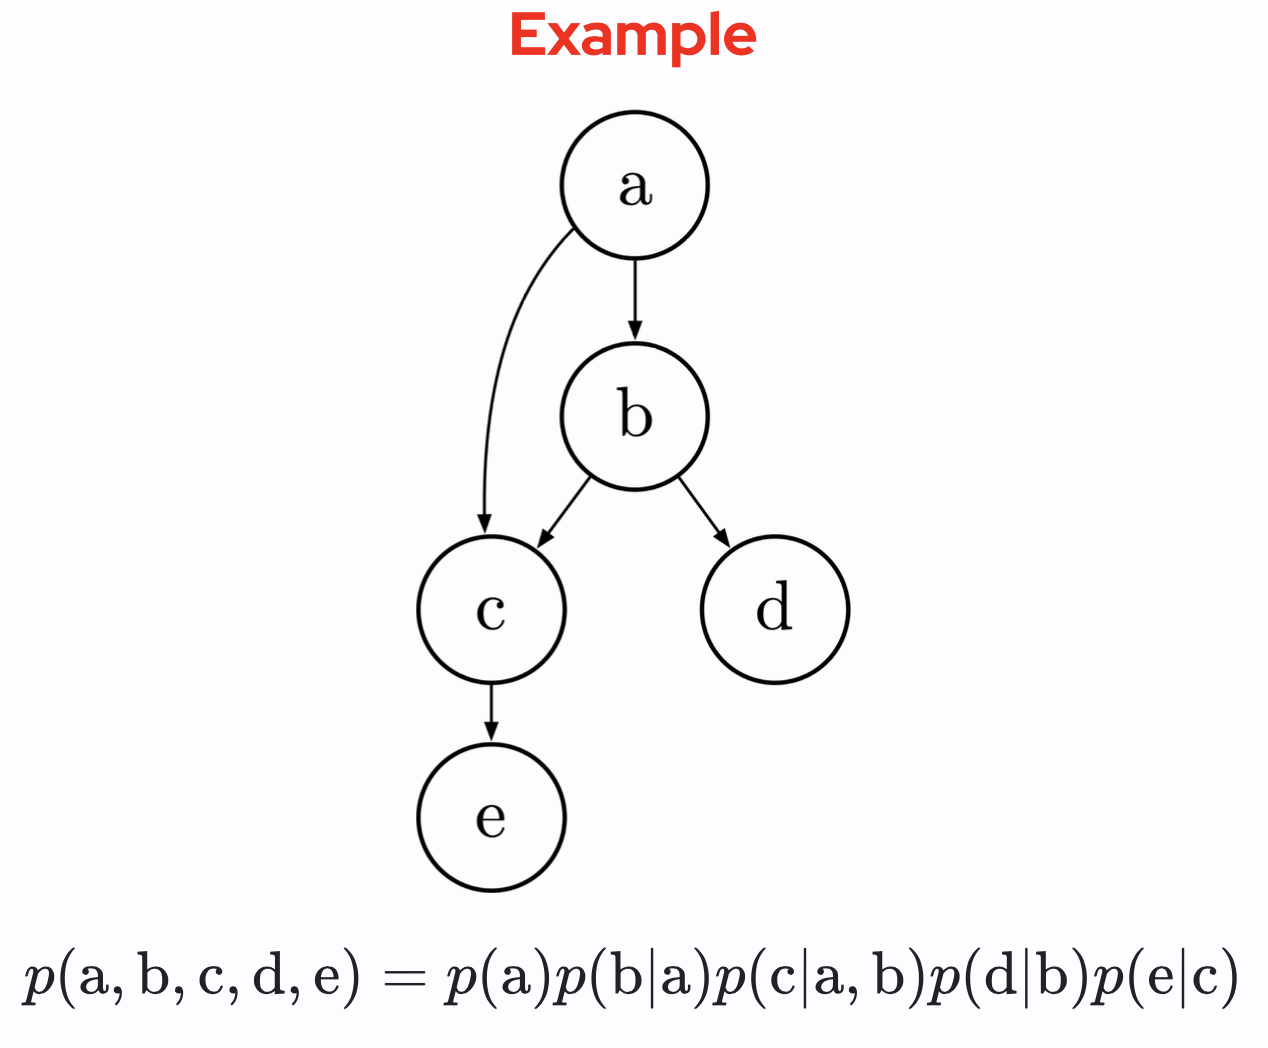
\includegraphics[scale=.5]{images/prerequisites/graphModelDir.png}
    \centering
\end{figure}
\newpage
\paragraph{Modelli indiretti.} Utilizzano grafi con archi indiretti. Rappresentano la fattorizzazione utilizzando un insieme di funzioni (non necessario né comune che siano distribuzioni probabilistiche):
\begin{itemize}
    \item c'è un fattore $\phi^{i}$ per ogni clique\footnote{sottografo completamente connesso.} $\mathcal{C}^{(i)}$ del grafo;
    \item la fattorizzazione è il prodotto normalizzato di tutti i fattori.
\end{itemize}
\begin{equation}
    p(\text{x})=\frac{1}{Z}\prod_i\phi^{(i)}(\mathcal{C}^{(i)}),
\end{equation}
con $Z=\sum_{x\in\text{x}}\prod_i\phi^{(i)}(\mathcal{C}^{(i)})$ fattore di normalizzazione.
\begin{figure}[!h]
    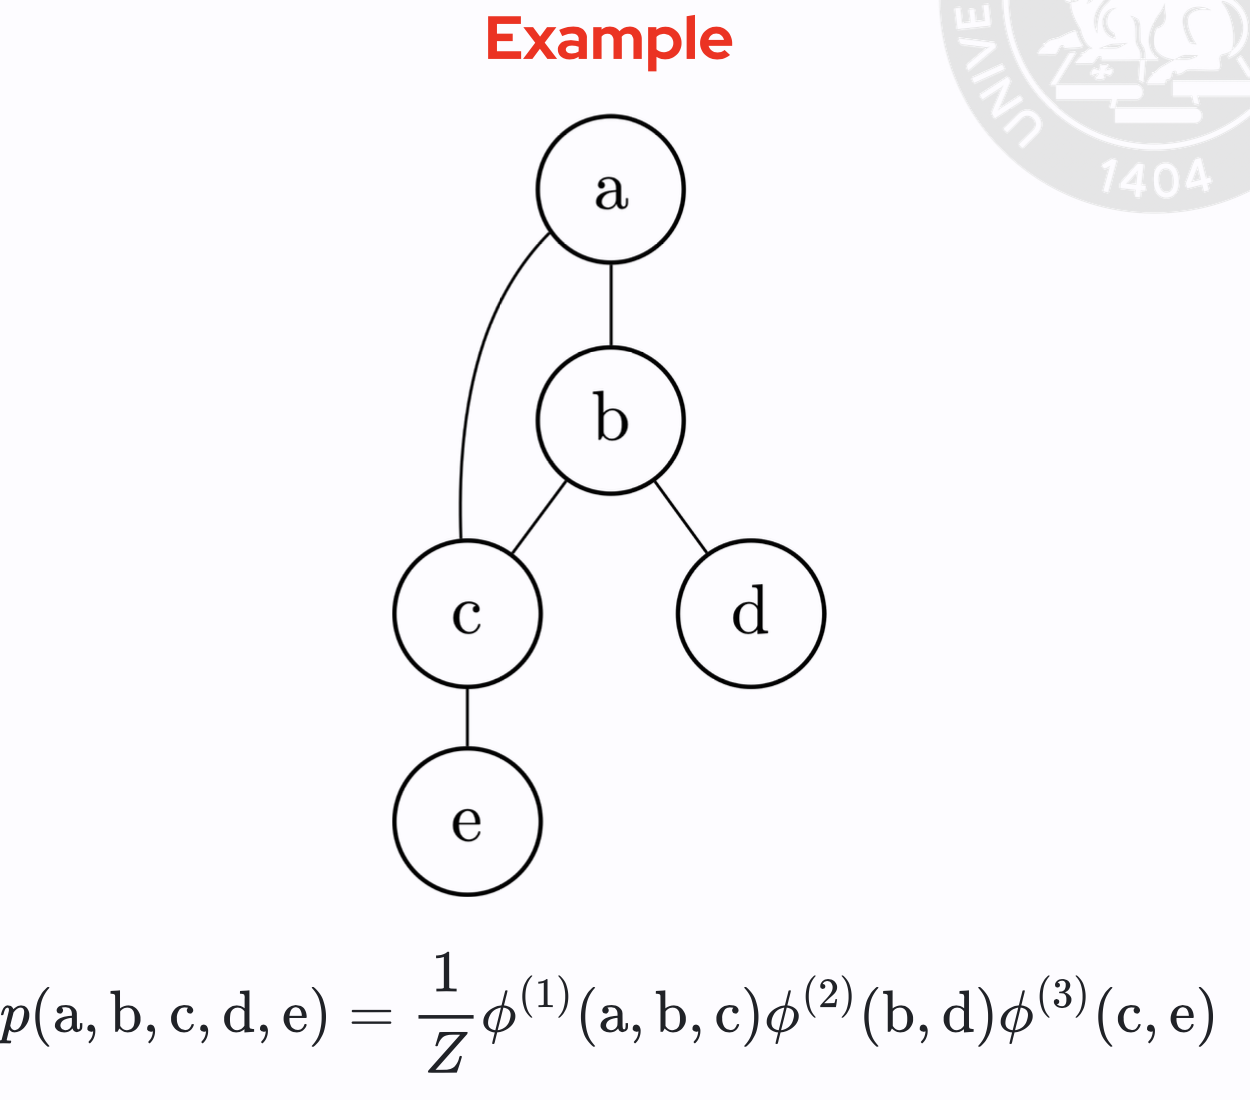
\includegraphics[scale=.5]{images/prerequisites/graphModelUnd.png}
    \centering
\end{figure}
\newpage